% -*- Mode:TeX -*-

%% The documentclass options along with the pagestyle can be used to generate
%% a technical report, a draft copy, or a regular thesis. You may need to
%% re-specify the pagestyle after you \include cover.tex. For more
%% information, see the first few lines of mitthesis.cls. 

%\documentclass[12pt,vi,twoside]{mitthesis}
%%
%%  If you want your thesis copyright to you instead of MIT, use the
%%  ``vi'' option, as above.
%%
%\documentclass[12pt,twoside,leftblank]{mitthesis}
%%
%% If you want blank pages before new chapters to be labelled ``This
%% Page Intentionally Left Blank'', use the ``leftblank'' option, as
%% above. 

% TODO: this line was modified from twoside to oneside
% to have less blank pages
% \documentclass[12pt,twoside]{mitthesis}

\documentclass[12pt,oneside]{mitthesis}
\usepackage{lgrind}
\usepackage{epigraph}
%% These have been added at the request of the MIT Libraries, because
%% some PDF conversions mess up the ligatures.  -LB, 1/22/2014
\usepackage{cmap}
\usepackage[T1]{fontenc}
\usepackage[main=english]{babel}
% \usepackage{glossaries}
% \usepackage[toc]{glossaries}
\usepackage[acronym, toc]{glossaries}
\usepackage{graphicx}
\graphicspath{ {./} }
\usepackage{listings}
\usepackage{color}
\usepackage{xurl}
\usepackage[skip=2pt]{caption}
\usepackage{diagbox}
\usepackage[pdfborder={0 0 0}, breaklinks]{hyperref}
\usepackage{pdfpages}
\usepackage{csquotes}
\usepackage[a-1b]{pdfx}
\usepackage{hyperref}
% \usepackage{pdfcomment}
% \usepackage{biblatex}
% \addbibresource{main.bib}
% \bibliography{main.bib}
% begin section from https://stackoverflow.com/a/3175141
\definecolor{dkgreen}{rgb}{0,0.6,0}
\definecolor{gray}{rgb}{0.5,0.5,0.5}
\definecolor{mauve}{rgb}{0.58,0,0.82}
\lstset{frame=tb,
  language=Java,
  aboveskip=3mm,
  belowskip=3mm,
  showstringspaces=false,
  columns=flexible,
  basicstyle={\small\ttfamily},
  numbers=none,
  numberstyle=\tiny\color{gray},
  keywordstyle=\color{blue},
  commentstyle=\color{dkgreen},
  stringstyle=\color{mauve},
  breaklines=true,
  breakatwhitespace=true,
  tabsize=3
}
% end section from https://stackoverflow.com/a/3175141
\makeglossaries

\newacronym{AI}{AI}{Artificial intelligence}

\newacronym{BLE}{BLE}{Bluetooth Low Energy}

\newacronym{DIY}{DIY}{Do it yourself}

\newacronym{ITP}{ITP}{Interactive Telecommunications Program}

\newacronym{MCU}{MCU}{Microcontroller unit}

\newacronym{MIDI}{MIDI}{Musical Instrument Digital Interface}

\newacronym{MIT}{MIT}{Massachusetts Institute of Technology}

\newacronym{ML}{ML}{Machine learning}

\newacronym{NYU}{NYU}{New York University}

\newacronym{OSS}{OSS}{Open source software}

\newglossaryentry{Arduino}
{
    name=Arduino,
    description={A microcontroller}
}

\pagestyle{plain}

%% This bit allows you to either specify only the files which you wish to
%% process, or `all' to process all files which you \include.
%% Krishna Sethuraman (1990).

%\typein [\files]{Enter file names to process, (chap1,chap2 ...), or `all' to process all files:}
\def\all{all}
\ifx\files\all \typeout{Including all files.} \else %\typeout{Including only \files.} \includeonly{\files} \fi

\begin{document}

% -*-latex-*-

\title{Tiny trainable instruments}

\author{Aarón Montoya-Moraga}
\prevdegrees{B.S., Pontificia Universidad Católica de Chile (2014) \\
M.P.S, New York University (2017)}

\department{Program of Media Arts and Sciences}

\degree{Master of Science in Media Arts and Sciences}

% As of the 2007-08 academic year, valid degree months are September, 
% February, or June.  The default is June.
\degreemonth{September}
\degreeyear{2021}
\thesisdate{September 2021}

%% By default, the thesis will be copyrighted to MIT.  If you need to copyright
%% the thesis to yourself, just specify the `vi' documentclass option.  If for
%% some reason you want to exactly specify the copyright notice text, you can
%% use the \copyrightnoticetext command.  
%\copyrightnoticetext{\copyright IBM, 1990.  Do not open till Xmas.}

% If there is more than one supervisor, use the \supervisor command
% once for each.
\supervisor{Tod Machover}{Muriel R. Cooper Professor of Music and Media}

\chairman{Tod Machover}{Academic Head, Program in Media Arts and Sciences}

\maketitle

% The abstractpage environment sets up everything on the page except
% the text itself.  The title and other header material are put at the
% top of the page, and the supervisors are listed at the bottom.  A
% new page is begun both before and after.  Of course, an abstract may
% be more than one page itself.  If you need more control over the
% format of the page, you can use the abstract environment, which puts
% the word "Abstract" at the beginning and single spaces its text.

%% You can either \input (*not* \include) your abstract file, or you can put
%% the text of the abstract directly between the \begin{abstractpage} and
%% \end{abstractpage} commands.

% First copy: start a new page, and save the page number.
\cleardoublepage
% Uncomment the next line if you do NOT want a page number on your
% abstract and acknowledgments pages.
% \pagestyle{empty}
\setcounter{savepage}{\thepage}
\begin{abstractpage}
% $Log: abstract.tex,v $
% Revision 1.1  93/05/14  14:56:25  starflt
% Initial revision
% 
% Revision 1.1  90/05/04  10:41:01  lwvanels
% Initial revision
%
%
%% The text of your abstract and nothing else (other than comments) goes here.
%% It will be single-spaced and the rest of the text that is supposed to go on
%% the abstract page will be generated by the abstractpage environment.  This
%% file should be \input (not \include 'd) from cover.tex.
How can we build flexible and reusable multimedia instruments that we can train instead of program? How can we build and publish our own personal databases for artistic purposes? What are the new choreographies and techniques that machine learning running on microcontrollers offer for artists and activists?

 \emph{Tiny trainable instruments} is a collection of multimedia devices, running machine learning algorithms on microcontrollers, for artistic purposes. It includes techniques for capturing data, building databases, training machine learning models, and deploying on microcontrollers. The software library created for this project allows for the creation of instruments that react to different inputs, including color, gesture, and speech, to control different multimedia outputs, including sound, light, and movement, using machine learning and embedded sensors.

This thesis has a strong emphasis on open source software and artificial intelligence ethis, and includes all the steps on creating these bridges between machine learning and media arts, that are respectful of privacy and consent because of their offline and off-the-grid nature.

\end{abstractpage}

% Additional copy: start a new page, and reset the page number.  This way,
% the second copy of the abstract is not counted as separate pages.
% Uncomment the next 6 lines if you need two copies of the abstract
% page.
% \setcounter{page}{\thesavepage}
% \begin{abstractpage}
% % $Log: abstract.tex,v $
% Revision 1.1  93/05/14  14:56:25  starflt
% Initial revision
% 
% Revision 1.1  90/05/04  10:41:01  lwvanels
% Initial revision
%
%
%% The text of your abstract and nothing else (other than comments) goes here.
%% It will be single-spaced and the rest of the text that is supposed to go on
%% the abstract page will be generated by the abstractpage environment.  This
%% file should be \input (not \include 'd) from cover.tex.
How can we build flexible and reusable multimedia instruments that we can train instead of program? How can we build and publish our own personal databases for artistic purposes? What are the new choreographies and techniques that machine learning running on microcontrollers offer for artists and activists?

 \emph{Tiny trainable instruments} is a collection of multimedia devices, running machine learning algorithms on microcontrollers, for artistic purposes. It includes techniques for capturing data, building databases, training machine learning models, and deploying on microcontrollers. The software library created for this project allows for the creation of instruments that react to different inputs, including color, gesture, and speech, to control different multimedia outputs, including sound, light, and movement, using machine learning and embedded sensors.

This thesis has a strong emphasis on open source software and artificial intelligence ethis, and includes all the steps on creating these bridges between machine learning and media arts, that are respectful of privacy and consent because of their offline and off-the-grid nature.

% \end{abstractpage}

\cleardoublepage

\section*{Acknowledgments}

This thesis could not have been possible with the support of these wonderful people, in alphabetical order:

\sloppy{Aaron, Agnis, Aillaly, Alexandra, Alonso, Ana María, Andrea, Andrew, Baltazar, Beatriz, Belén, Benjamín, Bernardita, Braulio, Camila, Camilo, Carla, Carmelo, Carolina, Casey, Catalina, Charles, Christian, Claudia, Corbin, Cynthia, Daniel, Daniella, Devora, Dorothy, Erik, Euge, Felipe, Fernanda, Francesca, Francisco, Gabriela, Gaurav, Guillermo, Hannah, Jasmine, Javiera, Jen, Jennifer, Jorge, José, Juan, Julian, Juniper, Karina, Karsten, Kathy, Katya, Lauren, Lily, Lindsey, Lisa, Luna, Mahy, Manaswi, Marco, Margarita, María José, Martin, Maxwell, Mel*, Mitchel, Monica, Namira, Natalia, Natalie, Nathier, Newén, Nicolás, Nicole, Nikhil, Nouf, Nushin, Olivia, Pablo, Patricio, Pedro, Peter, Priscilla, Rafael, Raúl, Rebecca, Rébecca, Renata, Ricardo, Rodrigo, Rosalie, Roy, Russell, Ruta, Sankalp, Sasha, Sayén, Sean, Sebastián, Sejo, Shir, Sofía, Sokio, Soledad, Tiri, TK, Tod, Tom, Verónica, Víctor, Victoria, Viniyata, Will, Wipawe, Yuan, Yuli, Yusuf, Zach}

%%%%%%%%%%%%%%%%%%%%%%%%%%%%%%%%%%%%%%%%%%%%%%%%%%%%%%%%%%%%%%%%%%%%%%
% -*-latex-*-

% % -*- Mode:TeX -*-
%
% If you choose not to use the "titlepage" environment, a \newpage
% commands, and several \vspace{\fill} commands may be necessary to
% achieve the required spacing.  The \signature command is defined in
% the "mitthesis" class

\begin{titlepage}
\begin{large}

% \signaturepage

% This master thesis has been examined by a Committee of the Department
% of Media Arts and Sciences as follows:

% \signature{Professor Tod Machover}{Thesis advisor \\
%    Muriel R. Cooper Professor of Music and Media}

% \signature{Professor Zach Lieberman}{Thesis reader \\
%    Adjunct Associate Professor of Media Arts and Sciences}

% \signature{Professor Mitchel Resnick}{Thesis reader \\
%    LEGO Papert Professor of Learning Research}
\end{large}
\end{titlepage}

\pagestyle{plain}
  % -*- Mode:TeX -*-
%% This file simply contains the commands that actually generate the table of
%% contents and lists of figures and tables.  You can omit any or all of
%% these files by simply taking out the appropriate command.  For more
%% information on these files, see appendix C.3.3 of the LaTeX manual. 
\tableofcontents
% \newpage
\printglossaries
% \newpage
\listoffigures
% \newpage
\listoftables

\chapter{Introduction}

\epigraph{Me caí, me paré, caminé, me subí \\ me fui contra la corriente \\ y también me perdí}{Soy Yo \\ Bomba Estéreo, 2015}

\section{Context}

This thesis is the capstone project of my Master's program between the academic years 2019-2021 in the Media Arts and Sciences program at the MIT Media Lab, where I am a Research Assistant in the Opera of the Future and Future Sketches groups.

This thesis is a collection of media arts instruments made with microcontrollers and \acrfull{ML}, with a strong emphasis on \acrfull{AI} ethics and \acrfull{DIY} methods. Its main audience - besides the academic one - is beginners and artists, and it is my hope that this work can inspire a new generation of instrument makers, artists, designers, educators, programmers, policy makers, activists, and enthusiasts.

\begin{figure}[ht]
  \centering
  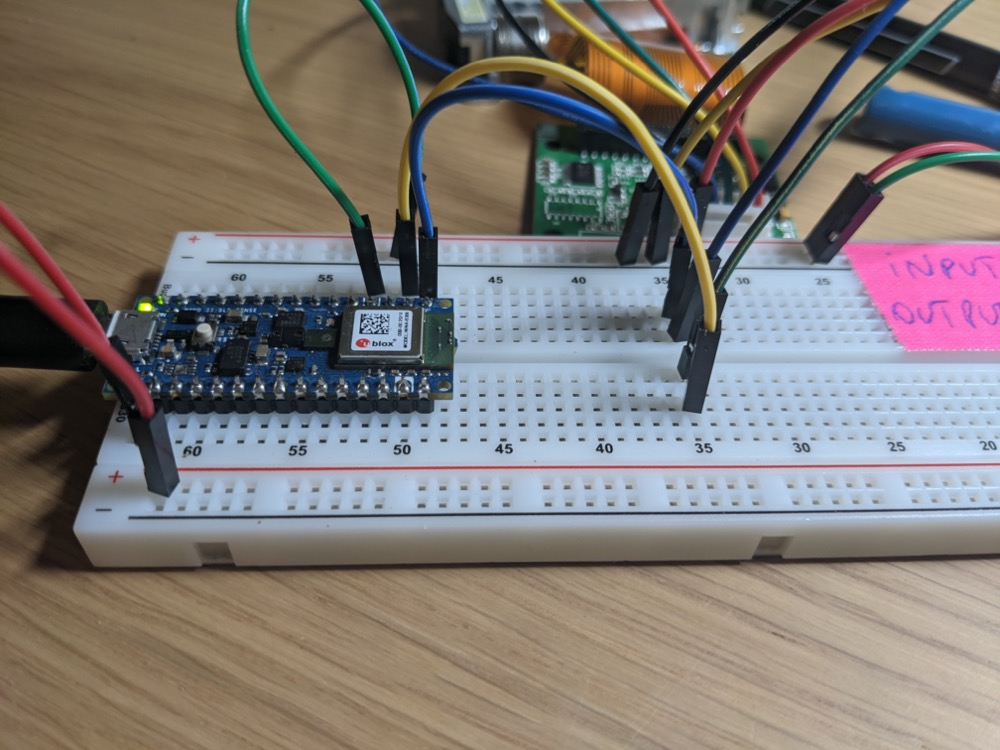
\includegraphics[width=0.75\linewidth,height=0.25\textheight,keepaspectratio]{images/tiny-trainable-instruments-early-protoype.jpg}
  \caption{Early prototype of Tiny Trainable Instruments}
  \caption*{Picture taken by myself}
  \label{fig:tiny-trainable-instruments-early-protoype}
\end{figure}

\acrshort{ML} has several barriers of entry, including cost, complexity, and difficulty. Since my practice is based on sharing and working openly with different communities, I am not a fan of the current state of industrial \acrshort{ML} that relies on proprietary software and hardware. This tends to happen because their ML models are aiming for high precision and need to be trained for long periods of time, using expensive non-open computational resources, with huge datasets that often are scraped from the internet without the explicit consent of users, and representing - in my view - a byproduct of surveillance capitalism.

\begin{figure}[ht]
  \centering
  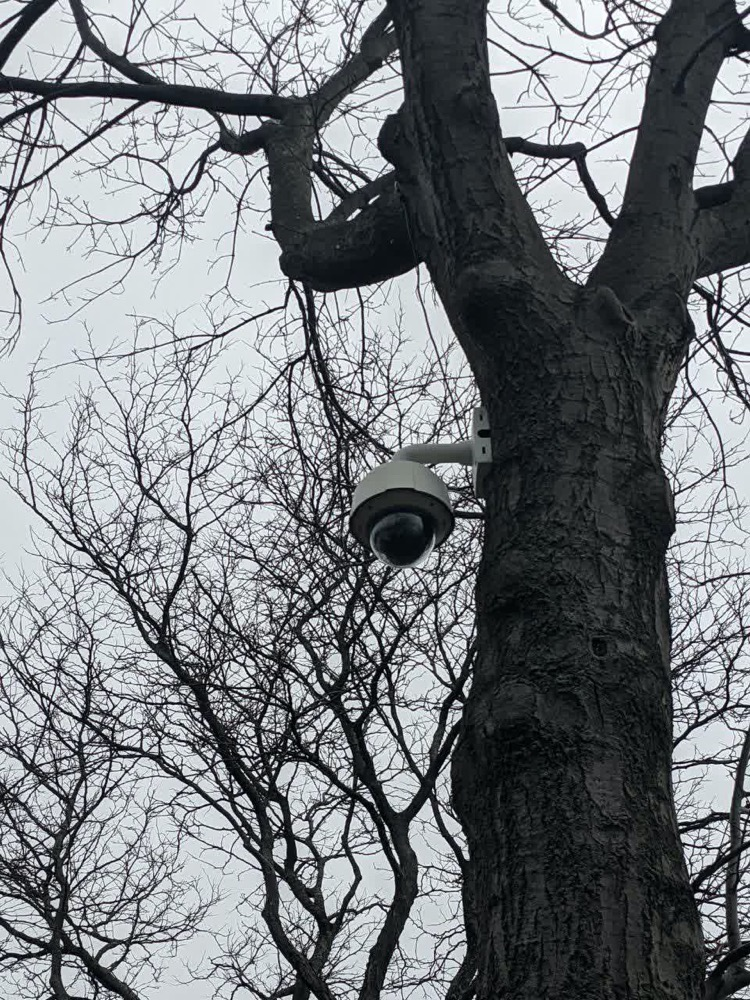
\includegraphics[width=0.75\linewidth,height=0.30\textheight,keepaspectratio]{images/surveillance-camera-tree.jpg}
  \caption{Surveillance camera in a park in Boston MA}
  \caption*{Picture taken by myself}
  \label{fig:surveillance-camera-tree}
\end{figure}

The release of the library Arduino TensorFlow Lite Micro in late 2019 \cite{google-tensorflow-lite-micro-arduino} made me aware of the \emph{tiny \acrshort{ML} field}, a subset of \acrshort{ML} that focuses on hardware and software able to run calculations both on-device and with low power, a stark contrast to many industrial \acrshort{ML} applications. The tutorials published by Arduino \cite{arduino-tensorflow-fruit-identification} showed how to build your own database to detect colors and gestures using a microcontroller, and I decided to make this thesis an artistic exploration of these emerging techniques.

One aspect that deeply resonated with me was \textbf{data agency}, and being in control of your own data, in particular its capture, storage, publication, and use. In this thesis I propose the microcontroller as a way of building our own databases and deploying our models to bypass any corporate or government surveillance. During this year and more of pandemic lockdown context, I have found myself several times working alone in my room, capturing data of myself and my living environment, and then building databases for other people to use, in a way that reminds of one of my favorite artists and activists, Ai Weiwei, who in 2012 - while facing government surveillance - decided to livestream from his house \cite{website-forbes-ai-weiwei-cam}. I also see this today as a way of reclaiming data agency.

\begin{figure}[ht]
  \centering
  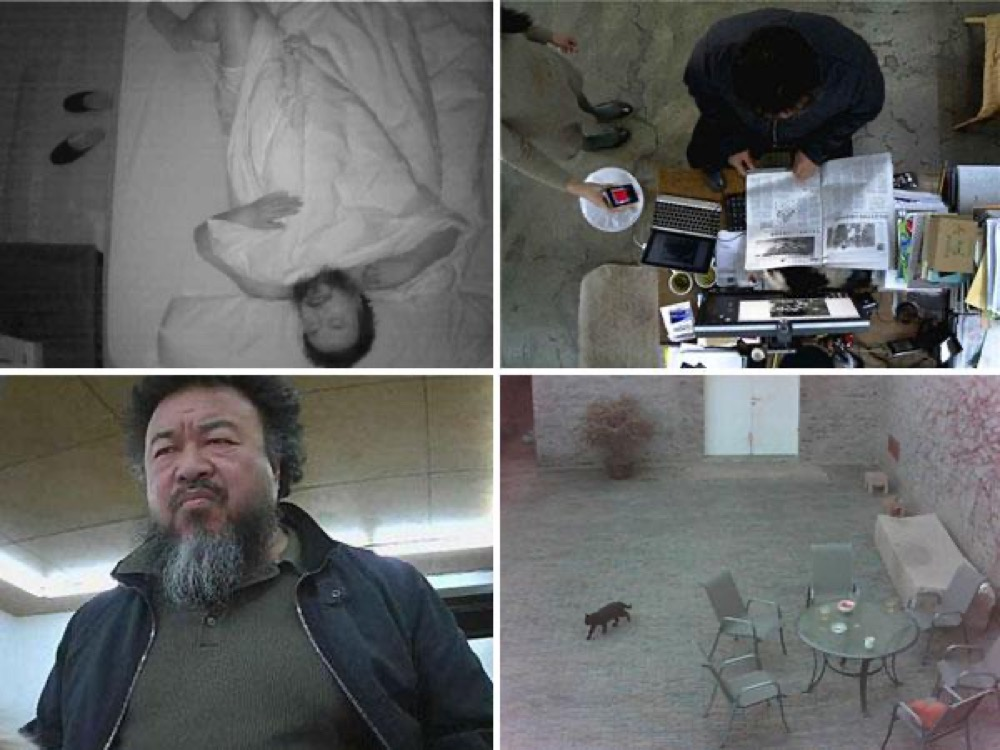
\includegraphics[width=0.75\linewidth,height=0.30\textheight,keepaspectratio]{images/weiweicam.jpg}
  \caption{Weiweicam, by Ai Weiwei, 2012}
  \caption*{Retrieved from \cite{website-forbes-ai-weiwei-cam}}
  \label{fig:weiweicam}
\end{figure}

I am an underrepresented minority in the USA, and it often happens that supposedly automatic neutral technologies fail to detect me. Here is an example of the popular software Zoom, where I spoke out loud: "This is a test to show that Zoom speech to text transcription does not work with my voice because of my accent." Indeed the words "Zoom" and "voice" were transcribed as "soon" and "boys", respectively.

\begin{figure}[ht]
  \centering
  
\includegraphics[width=0.75\linewidth,height=0.25\textheight,keepaspectratio]{images/zoom-introduction.jpg}
  \caption{Screen capture of speech-to-text on Zoom, introduction}
  \caption*{Screen capture by myself}
  \label{fig:zoom-voice}
\end{figure}

Here is a further experiment with more unusual words, the names of the members of my thesis committee: Tod Machover, Mitchel Resnick, and Zach Lieberman, where the transcription had even more errors.

\begin{figure}[ht]
  \centering
  
\includegraphics[width=0.75\linewidth,height=0.25\textheight,keepaspectratio]{images/zoom-committee.jpg}
  \caption{Screen capture of speech to text on Zoom, committee}
  \caption*{Screen capture by myself}
  \label{fig:zoom-committee}
\end{figure}

Despite these \acrshort{ML} algorithms being promoted by corporations and governments as unbiased and effective, most probably these algorithms have never been exposed to Chilean people with my accent, so they fail. Because of these errors, but more importantly because of not wanting to renounce my privacy, I routinely turn off voice assistants and text completion in my devices (if you have interacted with me over text, I typed every single character :)).

These examples do not affect me negatively, but these algorithmic decisions can easily have devastating effects in equity and discrimination. A famous example of this was the scrapped internal recruiting tool that Amazon developed with \acrshort{AI}, which systematically discriminated against women applicants, thus in fact reproducing and amplifying the existing biases of their own hiring teams\cite{website-reuters-news-amazon-ai-bias}. Researcher Timnit Gebru has also published about the dangerous bias and ecological impact of recent language models, \cite{wired-timnit-gebru-google}.

\begin{figure}[ht]
  \centering
  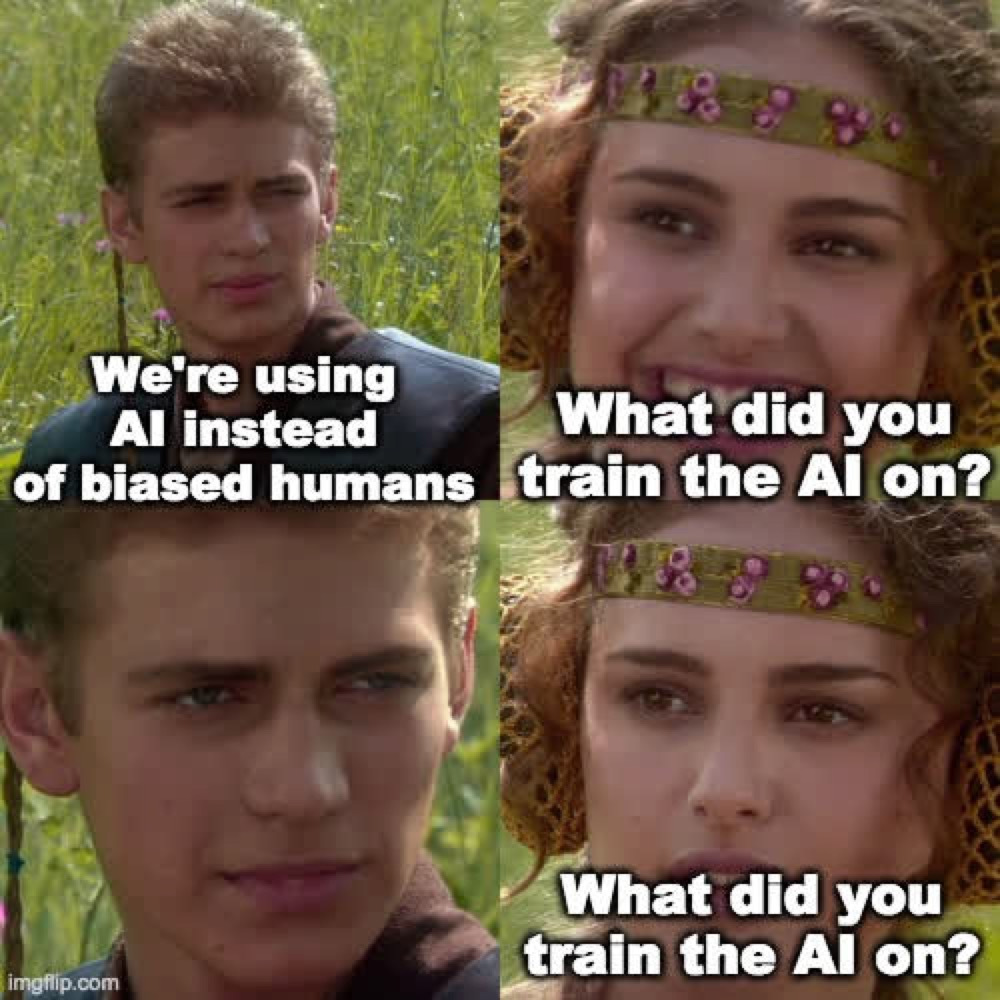
\includegraphics[width=0.75\linewidth,height=0.40\textheight,keepaspectratio]{images/meme-star-wars.jpg}
  \caption{Meme about biased data}
  \caption*{Retrieved from \cite{website-twitter-janellecshane-meme}}
  \label{fig:meme-star-wars}
\end{figure}

Sadly, we often cannot turn off or opt out of these computational or \acrshort{AI} systems. We should in fact be able to, because there is even more at stake than losing our privacy! We could be subjected to harmful \textbf{algorithmic bias}, as the Algorithmic Justice League \cite{website-algorithmic-justice-league} explains on their website:

\begin{displayquote}
In today’s world, AI systems are used to decide who gets hired, the quality of medical treatment we receive, and whether we become a suspect in a police investigation. While these tools show great promise, they can also harm vulnerable and marginalized people, and threaten civil rights. Unchecked, unregulated and, at times, unwanted, AI systems can amplify racism, sexism, ableism, and other forms of discrimination.
\end{displayquote}

I highly recommend watching the Coded Bias documentary \cite{website-coded-bias} currently available on Netflix, to inform oneself about the important and necessary digital advocacy of the Algorithmic Justice League, who have helped me learn the language for navigating these important topics of civil rights.

The final catalyst that led me to this thesis happened a year ago, when I watched a video \cite{website-talk-technology-and-public-art-rafael-lozano-hemmer} of a conversation between artists Rafael Lozano-Hemmer and Dorothy Santos. At 36:28 in the video, Rafael says "Face recognition needs to be banned in all applications except art."

This was the perfect spark for starting to work on this project, inspiring me to make more accessible these computational techniques to beginners, enthusiasts, and educators. Despite the creative and artistic applications that I will show during this thesis, let's keep in mind that as \acrshort{ML} becomes cheaper and more pervasive, it is not the solution to all problems, and might not even be needed in many scenarios.

\begin{figure}[ht]
  \centering
  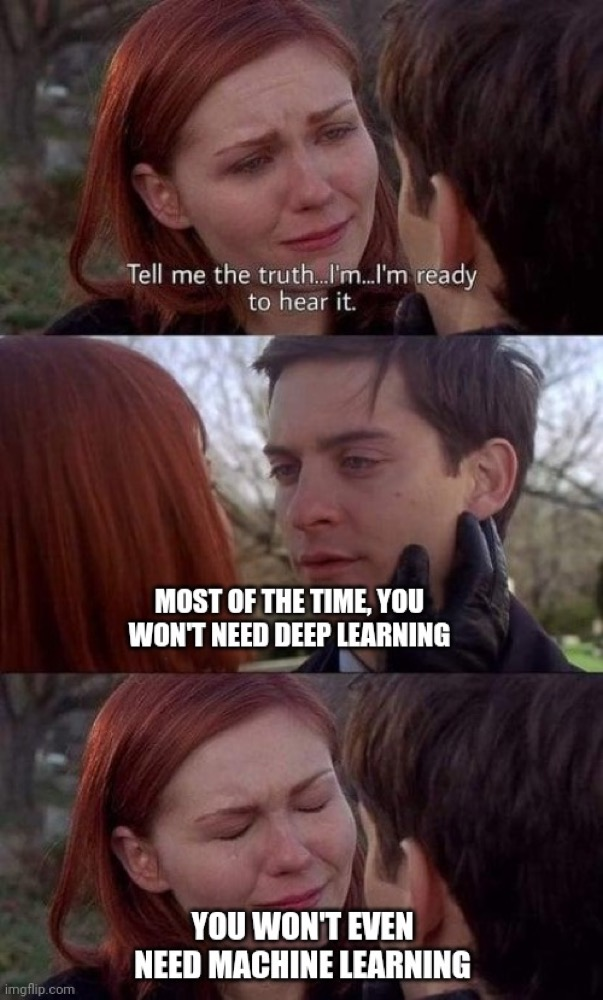
\includegraphics[width=0.75\linewidth,height=0.50\textheight,keepaspectratio]{images/meme-spider-man.jpg}
  \caption{Meme about need of machine learning}
  \caption*{Retrieved from \cite{website-twitter-dynamicwebpaige-meme}}
  \label{fig:meme-spider-man}
\end{figure}

In this 21st century artists have unprecedented access to tools for making more new tools and instruments, and I intend this thesis to be a foundation for a new generation of instrument makers for manipulating audiovisual material, using \acrshort{ML}. I think this approach is really exciting because it allows beginners and artists to train their instruments instead of programming them, by inputting data for tuning instead of having to write lines of code, and then fixing thresholds for changing their behavior.

\section{Objectives and dreams}

Infrastructure and cooperation are key to society. I love how I can bike on roads and hike on paths that were built as shared resources for the benefit of everyone. I hope this thesis work can be adopted by fellow artists and educators to create new instruments for arts, and to inspire critical and ethical thinking about \acrshort{AI}.

I am convinced there is a huge educational value in creating your own databases, and in this thesis I propose techniques and software so that people can build their own databases, in order to train models that are tailored to each person's voice or environment, instead of using widespread databases and their inherent biases. Also I hope this work will help appreciate the craft of making databases, or even the exploitation and problematic lack of consent behind them.

Finally, as a non-U.S. citizen subjected to all sorts of regulations during my studies here, as a programmer working with software under various licenses, and as a musician repurposing other people's work via sampling, I know first hand that navigating legal documents is very hard. As an anecdote, in 2010, GameStation added a soul clause to their terms of conditions as an April Fool's prank, making them legal owners of thousands of customers' souls \cite{website-huffpost-gamestation-soul-clause}. And in 2007, it was estimated that people would need around 250 hours every year to actually read the privacy policies shown to them \cite{article-cost-of-reading-privacy-policies}. That is why in this thesis I have tried my best to cite every work that I am either using as a building block, or that served as a direct or indirect inspiration.

I hope this work can be taken to the next level by others, through building a new generation of private and smart devices, like one of my first dreams, a drum machine I can talk to, and that would let me ask for different rhythms mid-performance, or let me use my body gestures to write poems.

\section{Thesis outline}

This thesis has cover the following chapters:

\begin{enumerate}
  \item Chapter 1 - Introduction: the context and summary of this thesis.
  \item Chapter 2 - Tiny Trainable Instruments: description of the design strategies for the software and hardware, description of the support team working on this thesis.
  \item Chapter 3 - Early experiments: my earlier work that led to this thesis, in the topics of media arts education, microcontrollers, and \acrshort{ML}, among others.
  \item Chapter 4 - Background and inspiration: work by other people which has informed my work.
  \item Chapter 5 - Project evaluation: user feedback, field notes.
  \item Chapter 6 - Conclusions and future work: next iterations of the instruments, and their proposed use for educators and artists.
  \end{enumerate}

\chapter{Early experiments}

\epigraph{And you may ask yourself \\ "Well\dots how did I get here?"}{Once in a Lifetime \\ Talking Heads, 1981}

In this chapter I showcase early experiments in the different fields I worked on for this thesis, with a strong focus on the different aspects of my education and artistic practice.  I include many of my breakthroughs and pitfalls that eventually led me to working on this thesis, in an open, detailed, celebratory, and critical narrative.

\section{Learning microcontrollers}

I learned how to program microcontrollers around 2010 in Chile as an undergraduate student of electrical engineering. I was taught how to program PIC microcontrollers with Microsoft's tools, including the operating system Windows and the C\# programming language. Around the same time, with my classmate Braulio we made our first project with an Arduino Uno microcontroller. It consisted of a robotic guitar tuner, where the Arduino detected the pitch of a string, analyzed the frequency, and then made a servo motor move the tuning gear of the string, in order to match the desired pitch.

\begin{figure}[ht]
  \centering
  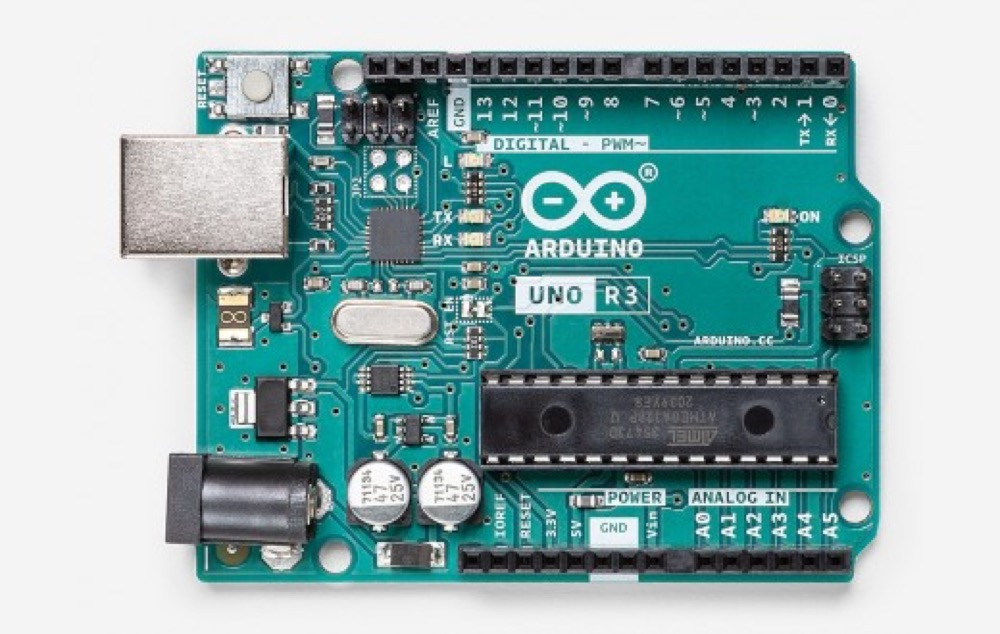
\includegraphics[width=0.75\linewidth,height=0.25\textheight,keepaspectratio]{images/arduino-uno.jpg}
  \caption{Arduino Uno microcontroller}
  \caption*{Retrieved from \cite{website-arduino-uno}}
  \label{fig:arduino-uno}
\end{figure}

Fast forward to 2013. For my undergraduate thesis I had to complete a capstone project and implement many low-level programming techniques, and Arduinos were not allowed because they were considered a shortcut. For this thesis I worked with my classmate Guillermo, and we built a robotic device with a \acrshort{PIC} microcontroller programmed with C\#. Our code was very specific to that particular chip and project, and hardly reusable or interesting for a wider audience.

Since graduation I haven't programmed with \acrshort{PIC} microcontrollers. I realized I wasn't excited about making one-off devices with non-reusable code that I couldn't share, or with having to use proprietary or bulky interfaces for writing or deploying my code. In contrast, Arduinos became a huge part of my practice, because of their low cost, open source nature, ease of programming and uploading the code with a generic USB cable, and because of the enormous and growing available documentation and user contributed libraries, which now also include the TinyTrainable library developed for this thesis project.

The Arduino ecosystem fostered many aspects of my practice, and now looking at it in retrospect, \textbf{I realize that what I love is not computers but computation}, making small machines that can crunch numbers for art, and making them openly and in collaboration with friends.

A huge argument that I see people on the internet making against Arduino microcontrollers, is that they are too expensive (around 30.00 USD) in comparison to the 1/10th of the cost of the bare bones chips and parts you need to build your own microcontroller unit. I am against this argument, since it invisibilizes the effort put in documentation by the Arduino community, and it also assumes that everybody is comfortable soldering and has advanced electronics degrees. Even if you factor in the cost of hours you need to make your own, it doesn't pay for itself. Obviously, I see the educational advantage of building your own things, but it's a slippery slope and it is discriminatory to think that if you build a project with an Arduino, it's not good because it's not from scratch. In fact, I think it's rude to say it's not worth it, as rude as complaining about someone buying bread and making fun of them for not buying the ingredients and cooking it themselves.

Another strong argument against Arduino microcontrollers is about efficiency: that Arduino is too high-level and over-bloated, and that applications and projects could be faster if you programmed in a lower-level language. I also see this argument when comparing different programming languages for graphic arts. Once again, knowing how to program with lower-level programming languages is amazing, and there is value and fun on it. But in my practice, I put a high value on my time and energy, and I'd rather make my code slower or less efficient so I can spend more time making art or resting.

I'd rather that we all have non-painful programming experiences, so that we can spend more time away from screens and making more art!

\section{Computer music and physical computing}

During undergrad studies, I took classes and did research with professors and computer musicians Rodrigo Cádiz and Patricio de la Cuadra. With them I learned the fundamentals of computer music, including languages such as Max and Pure Data, which I still use to this day. For a class project I created a spoon synthesizer with masking tape, cardboard, and a Makey Makey \cite{website-makey-makey}, a device created in 2010 by Eric Rosenbaum and Jay Silver from the MIT Media Lab's Lifelong Kindergarten research group. This was my first hands-on introduction to physical computing, as a way of building my own custom playful interfaces for manipulating sound with computers.
 
\begin{figure}[ht]
  \centering
  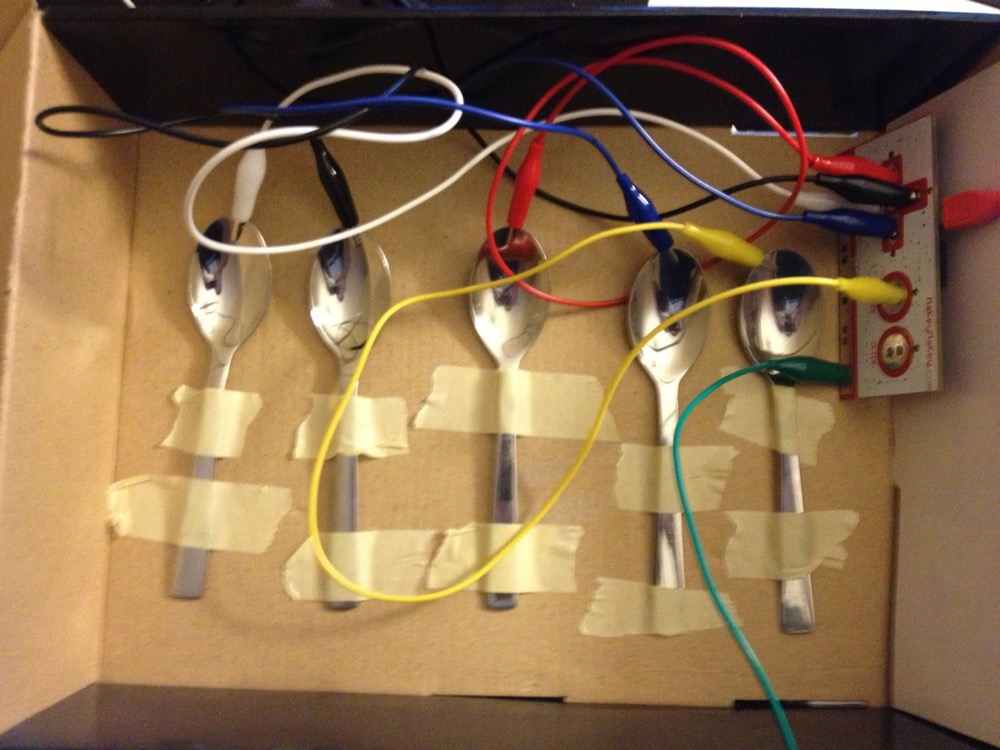
\includegraphics[width=0.75\linewidth,height=0.25\textheight,keepaspectratio]{images/makey-makey-spoons.jpg}
  \caption{Spoons and Makey Makey synthesizer}
  \caption*{Picture taken by myself}
  \label{fig:makey-makey-spoons}
\end{figure}

For this project I applied my practice as a guitar player, where I am constantly mixing and matching different devices on my pedalboard. This inspired me to make this flexible synthesizer with objects lying around me: spoons, masking tape, and cardboard. They also are forgiving, and I was able to change their physical position. The Makey Makey acted as an interface with the computer, where I could assign on the fly different sounds to each spoon.

In retrospect, this project was an amazing experience that followed Mitchel Resnick's 4 P's: it was a Passion Project that I built for Playing with my Peers, which is a constant in my artistic practice.

\section{Physical computing and more microcontrollers}

After graduation in 2013 I freelanced as a software and technology designer and developer for artists. I learned computer protocols and networks, and wrote custom software for live multimedia theater and music shows. Realizing that I wanted a bigger community of people to learn media arts with, I applied to New York University's Interactive Telecommunications Program (\acrshort{NYU} \acrshort{ITP}), where I joined as a graduate student in 2015. In my first semester, I took the class Introduction to Physical Computing \cite{website-nyu-itp-intro-physical-computing}, taught by one of Arduino's co-creators, Tom Igoe. Since I was already familiar with electronics and circuits, I focused on learning interface design, human computer interaction, open source hardware and software, and physical computing education.

During my research I was introduced to a wider ecosystem of microcontrollers beyond Arduino, that were made possible because of its open source nature and the community behind it. My favorite example is the Teensy by PJRC \cite{website-pjrc}, which captivated me by two main features: it can send and receive \acrshort{MIDI} over USB, and it has a powerful audio library that allows you to play audio samples, create effects, and process real time audio. With Teensy, I was able to make standalone projects in a way that before would have required me to use a full-fledged computer.

\begin{figure}[ht]
  \centering
  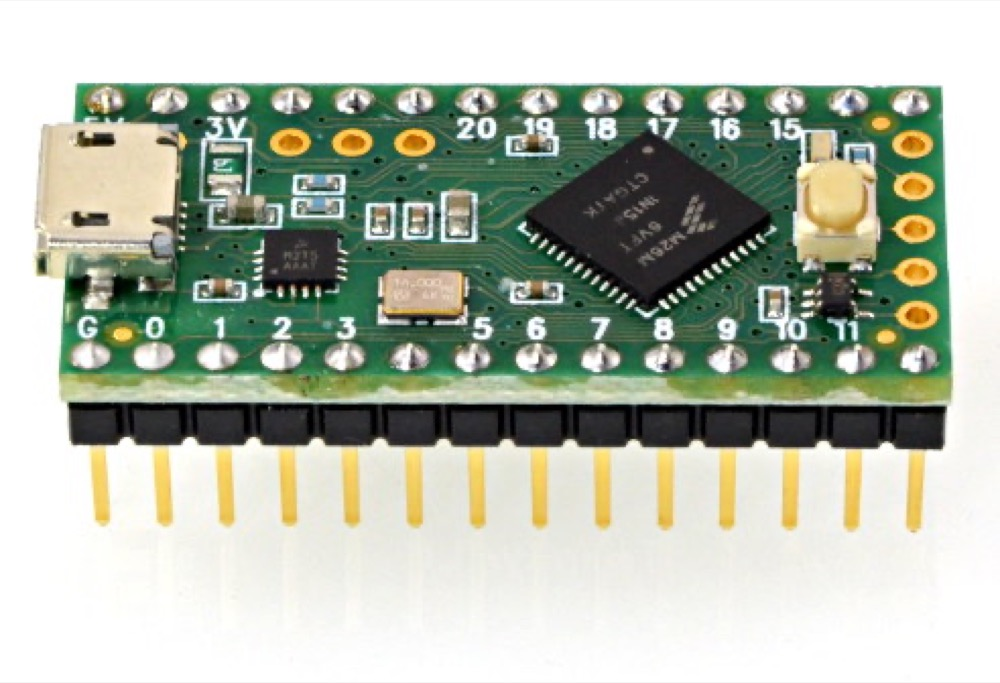
\includegraphics[width=0.75\linewidth,height=0.25\textheight,keepaspectratio]{images/pjrc-teensy-lc-with-pins.jpg}
  \caption{PJRC Teensy LC microcontroller with pins}
  \caption*{Retrieved from \cite{website-pjrc-teensy-lc-with-pins}}
  \label{fig:pjrc-teensy-lc-with-pins}
\end{figure}

\section{Processing, p5.js, Processing Foundation}

Processing \cite{website-processing} is an open source software written in Java, and it was started at the MIT Media Lab's Aesthetics and Computations group by Ben Fry and Casey Reas. Over the years I have learned Processing on my own, and through it, computer graphics and interactivity.

I was excited to learn more Processing in 2015 in my first semester at \acrshort{NYU} \acrshort{ITP}'s Introduction to Computational Media class, like it had been taught for around a decade. I consider myself lucky, because that year they replaced the curriculum in Processing with a new one based on p5.js, another software library supported by the Processing Foundation.

p5.js was created by Lauren McCarthy as a reinterpretation of Processing, using JavaScript instead of Java, to make art that runs on web browsers and over the internet. With p5.js I learned artistic and creative ways to program web applications, and this experience led me to focus on educational outreach with the Processing Foundation, which I will mention in the next section.

I was not only in awe of p5.js and Processing, but also of the people and the communities behind these software libraries. I took Lauren McCarthy's Performing User class \cite{website-nyu-itp-lauren-mccarthy-performing-user} at \acrshort{NYU} \acrshort{ITP}, and it was my favorite class during my Master's there. She fostered a safe space for us to explore societal and political implications of software, and it led me to add more of my personal convictions, and my body, to my artwork. This class inspired me to make \emph{its-ok-to-die} \cite{its-ok-to-die}: a self portrait, with a countdown timer to my projected death time according to the United Nations' estimates. The first version I did was a Processing app running on a Raspberry Pi computer, and I also ported it to p5.js for web access.

\begin{figure}[ht]
  \centering
  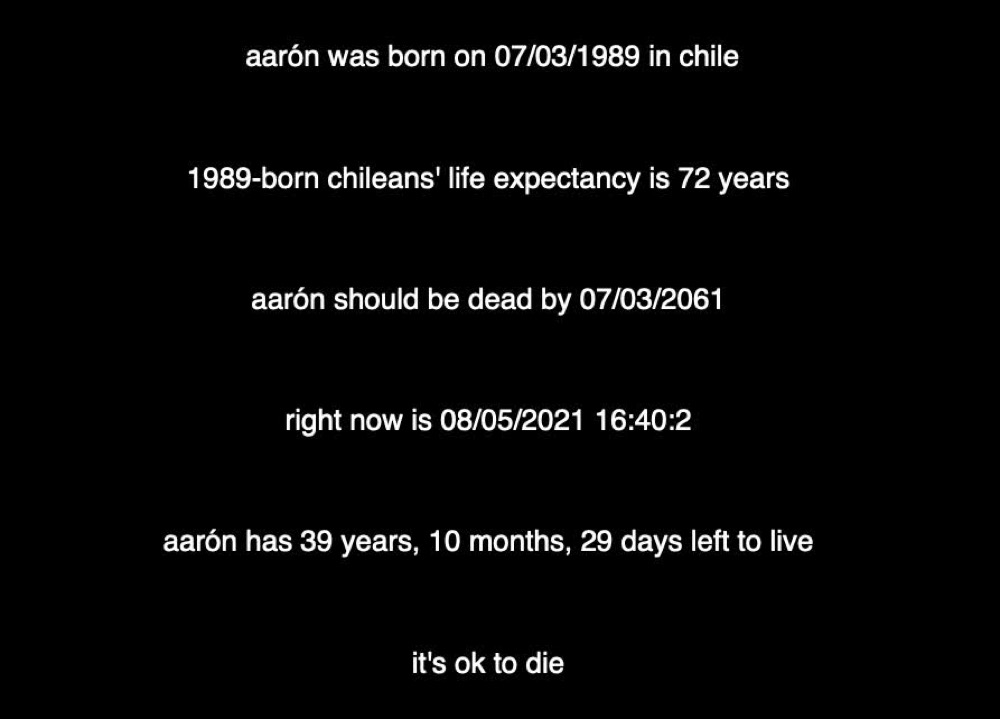
\includegraphics[width=0.75\linewidth,height=0.35\textheight,keepaspectratio]{images/its-ok-to-die-p5js.jpg}
  \caption{its-ok-to-die, on a browser with p5.js}
  \caption*{Screen capture by myself}
  \label{fig:its-ok-to-die-p5js}
\end{figure}

\begin{figure}[ht]
  \centering
  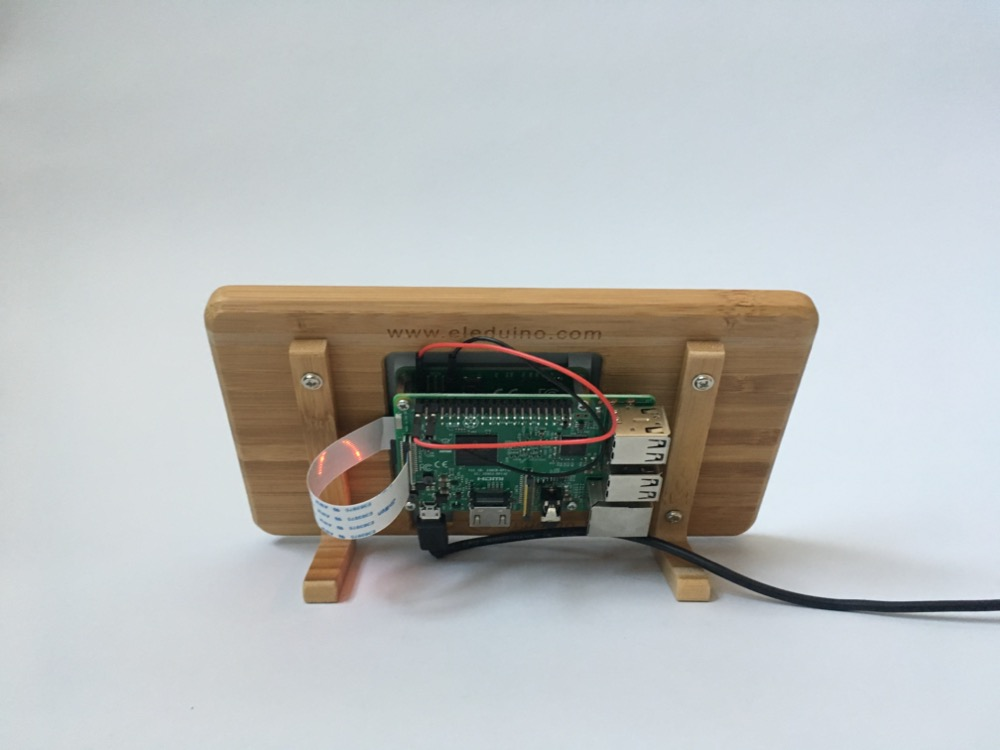
\includegraphics[width=0.75\linewidth,height=0.35\textheight,keepaspectratio]{images/its-ok-to-die-raspberry.jpg}
  \caption{its-ok-to-die, on a Raspberry Pi computer}
  \caption*{Picture taken by myself}
  \label{fig:its-ok-to-die-raspberry}
\end{figure}

\section{Teaching media arts}

While I was a student at \acrshort{NYU} \acrshort{ITP}, I was the recipient of two summer grants to work on an internationalization project of p5.js. Since my native language is Spanish, and I wanted to share all my passion for web programming with p5.js, I focused on translating the official p5.js website \cite{website-p5js-spanish} and book \cite{p5js-spanish-book} to Spanish, and teaching introductory workshops in Spanish in my home country, Chile. My main goal was to let people be able to learn and enjoy p5.js without having to first learn English. Since then, this project has been expanded to other languages, and I am still a contributor to p5.js.

Another reason why I wanted to teach and share p5.js is because still to this day their community statement \cite{website-p5js-community-statement} is one of my favorite documents, fostering an inclusive environment for artists. This document inspired the ml5.js community statement \cite{website-ml5js-community-statement}, a \acrshort{ML} library for arts created at \acrshort{NYU} \acrshort{ITP} with a strong emphasis on \acrshort{AI} ethics.

In my workshops and classes, when I have taught p5.js or ml5.js, I like to take a moment with my students to read the community statements, and also to read the source code, and show them the repositories where these libraries are developed. I think it is very educational to take a moment and acknowledge the work made by the community to build these libraries. I also like to point out that these libraries are not made out of scratch (Hennessy Youngman claims that in the arts, we ran out of scratch in the 1960s (\cite{hennessy-youngman-art-thoughtz-how-to-make-an-art}). p5.js is a wrapper for drawing and interactivity features of HTML5, and ml5.js is a wrapper of Google's TensorFlow.js library.

Another feature of my classes is that even though I always teach with a particular toolkit, I like to give students an overview of different alternatives that they can use to achieve similar results. I want my student to be able to work in an agnostic way; even if they don't continue using the tools I teach, they learn fundamentals of programming and arts. Since most of my recent workshops and classes have been short crash courses on complex topics, I make my best efforts to share additional resources with students so that they can continue learning on their own. This is the reason why I enjoy being a contributor and maintainer of documentation of open source projects. It is my way of giving back to the community of volunteers who has given me access to learning on my own over the years.

I hope that people find the documentation and writing of the TinyTrainable library useful, and that even if they don't end up using it, they learn fundamentals of programming, \acrshort{ML} ethics, and how to use the different outputs and protocols I showcase.

\section{Publishing libraries}

After years of working with different software libraries for arts, and publishing my code and teaching with it, I started packaging and writing my own software libraries, with the hope that people can reuse my code and learn from it. My first experiments were in the Python ecosystem, where I have published protestpy \cite{website-pypi-protestpy}, a library for creating protest material, and kaputtpy \cite{website-pypi-kaputtpy}, a library for ruining digital devices.

\begin{figure}[ht]
  \centering
  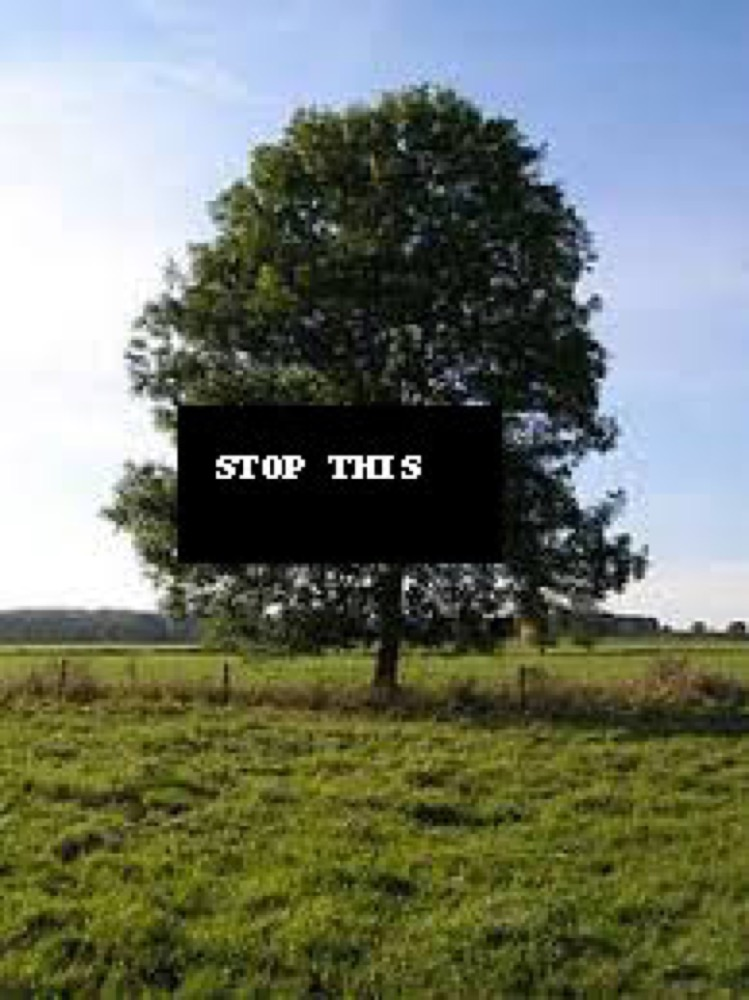
\includegraphics[width=0.75\linewidth,height=0.35\textheight,keepaspectratio]{images/protestpy.jpg}
  \caption{protestpy image for protesting against trees}
  \caption*{Screen capture by myself}
  \label{fig:protestpy-tree}
\end{figure}

Publishing my libraries so they can be installed with one-click or a command line, and making them depend on other libraries and languages, is for me an exercise in trust, and a way to give back to other artists what I have learned. It's my software version of building a skatepark or a hiking trail, it's infrastructure so that other people can use it for their own needs, mostly for fun and art :)

Apart from these software libraries, I have made small publishing experiments in other ecosystems, such as Max, Haskell, and Node.js, and the bulk of my work since 2016 is published as open source \gls{Git} repositories on my GitHub account at \url{https://github.com/montoyamoraga/}.

\begin{figure}[ht]
  \centering
  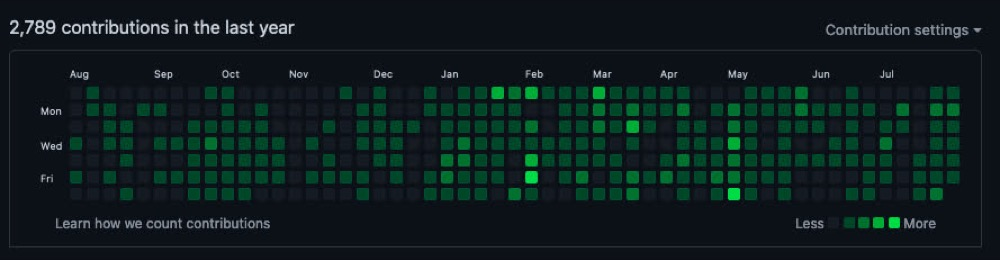
\includegraphics[width=0.80\linewidth,height=0.40\textheight,keepaspectratio]{images/github-contributions.jpg}
  \caption{GitHub contributions}
  \caption*{Screen capture by myself}
  \label{fig:github-contributions}
\end{figure}

TinyTrainable is my first library for hardware, and this experience has led me to publish libraries and releases for other projects I have been working on during this Master's, which I will continue to build after graduation.

\section{ML for arts}

My first project in \acrshort{ML} for arts was in 2016 with my \acrshort{NYU} \acrshort{ITP} classmate Corbin Ordel, who was a student at Gene Kogan \cite{website-gene-kogan}'s \acrshort{ML} for Artists class \cite{website-gene-kogan-machine-learning-for-artists}. Together we audited Rebecca Fiebrink\cite{website-rebecca-fiebrink}'s \acrshort{ML} online ML class on the Kadenze platform \cite{kadenze-ml-for-musicians-and-artists}, and learned her Wekinator \cite{website-wekinator} platform. As a final project for Gene's class, with Corbin we made the project Piano Die Hard, a digital sculpture consisting of a piano that is watching the trailer for the movie Die Hard, and every time it detects an explosion, it plays music as accompaniment.

\begin{figure}[ht]
  \centering
  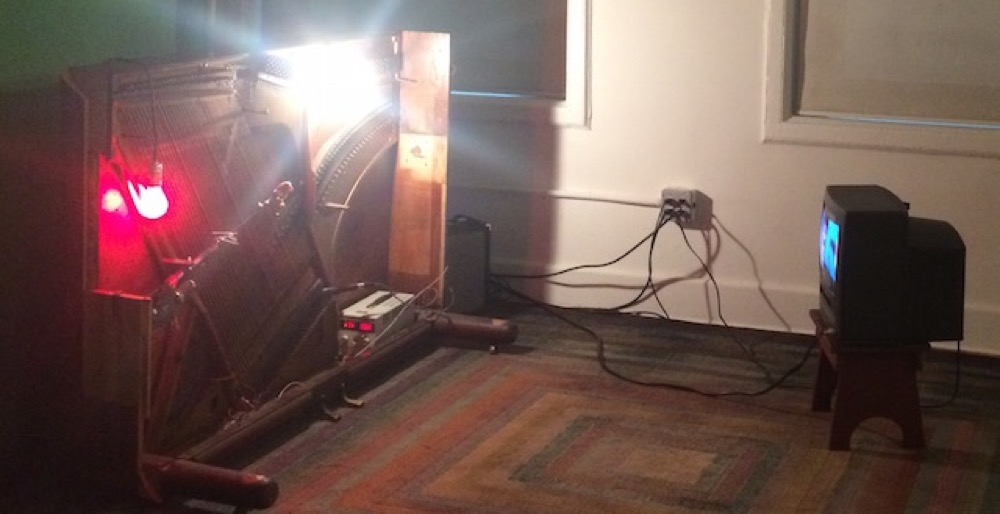
\includegraphics[width=0.80\linewidth,height=0.40\textheight,keepaspectratio]{images/piano-die-hard.jpg}
  \caption{Piano Die Hard}
  \caption*{Retrieved from \cite{website-alt-ai}}
  \label{fig:piano-die-hard}
\end{figure}

The technology stack for this project was very convoluted: a computer looped the trailer of the movie and fed it to an old TV and to an openFrameworks app. This app outputted statistical descriptors about the color of each picture frame, which were then sent to the Wekinator app, which decided with a \acrshort{k-NN} algorithm if the image was either an explosion or not. When it detected an explosion, it sent a control signal to an Arduino microcontroller, which moved a motor connected to a fishing rod and a kitchen utensil, which scratched the strings of the open carcass of an old piano every time there was an explosion.

The training of the model was made beforehand with a selection of 1980's movies, featuring scenes with and without explosions. This project was a direct inspiration for the color input of the TinyTrainable library, using also color data with a \acrshort{k-NN} algorithm. It's really fascinating for me to compress all of this complexity of five years ago, needing a computer and different apps, into a single microcontroller. I hope that everybody can enjoy this too!

After graduating from \acrshort{NYU} \acrshort{ITP} and working for one year as a research resident and graduate teaching assistant, I was exposed to many exciting developments in \acrshort{AI} and creativity, including witnessing the creation of the the ml5.js library, and the company RunwayML \cite{website-runwayml} founded by Cristóbal Valenzuela \cite{website-cristobal-valenzuela}, Alejandro Matamala \cite{website-alejandro-matamala}, and Anastasis Germanidis \cite{website-anastasis-germanidis}. Through this I became excited about the creative potential of \acrshort{ML}, so in 2018 I took a month-long intensive class at the School of Machines, Making \& Make-Believe \cite{website-school-of-machines} in Berlin, Germany, facilitated by Gene Kogan and Andreas Refsgaard \cite{website-andreas-refsgaard}, and organized by Rachel Uwa \cite{website-rachel-uwa}.

During this workshop I got a mix of excitement for the graphic and plastic possibilities that \acrshort{AI} allowed me, and frustration while working with databases. The algorithms I was trying to play with needed very specific requirements in terms of their data input, such as specific image resolution, file formats,  and file size. So even if I found an existing database, I had to do very tedious labor to adapt them. During this class my work focused on writing scripts to create custom databases with web \gls{scraping}, which you can find at this repository \url{https://github.com.montoyamoraga/scrapers}.

I learned web scraping as a student of artist Sam Lavigne. Sam is one of my role models, because he uses computation and comedy to address complex civic topics, including late capitalism, government surveillance and mass incarceration. Not only he makes amazing artwork, he also creates open source tools and teaches classes so that other artists and activists can learn powerful computational techniques.

\begin{figure}[ht]
  \centering
    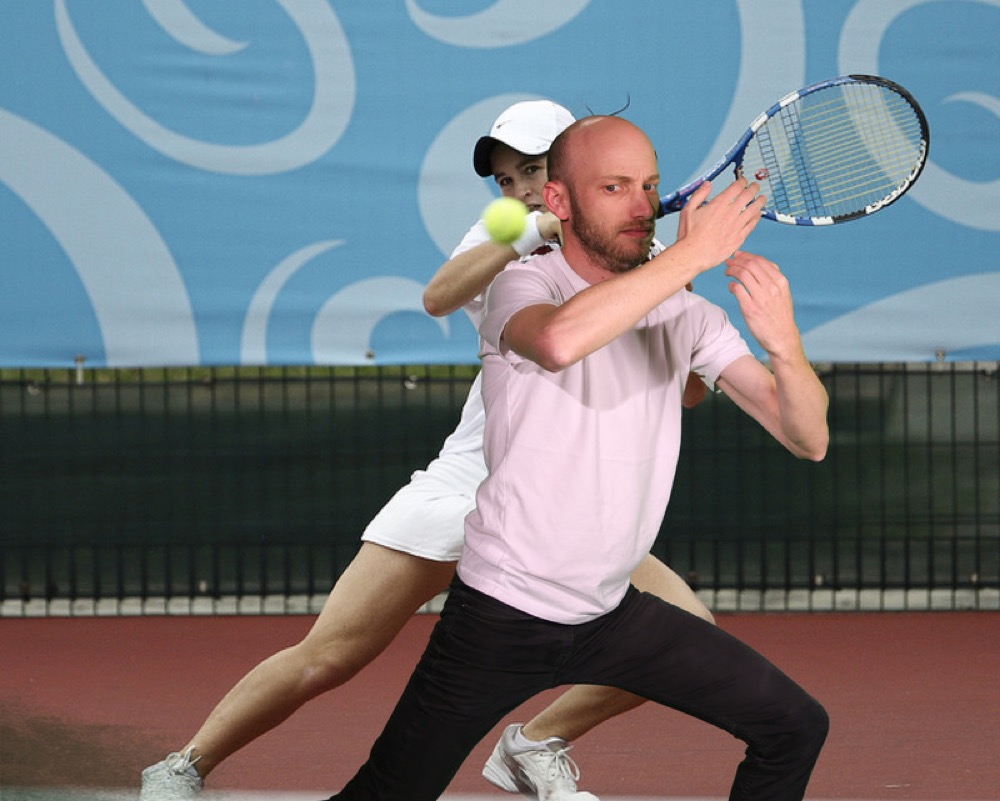
\includegraphics[width=0.75\linewidth,height=0.25\textheight,keepaspectratio]{images/sam-lavigne-training-poses.jpg}
  \caption{Sam Lavigne, Training Poses, 2018}
  \caption*{Retrieved from \cite{website-sam-lavigne-training-poses}}
  \label{fig:sam-lavigne-training-poses}
\end{figure}

I want to highlight his piece Training Poses (2018) \cite{website-sam-lavigne-training-poses}, a satirical response to the popular OpenPose \cite{website-openpose} library for body detection. Both of these projects use as source material Microsoft's \acrfull{COCO} database, consisting of thousands of images from Flickr, and annotated by workers on Amazon Mechanical Turk. This piece made me aware and worried of the existence of these enormous databases, and of the potential issues of consent and exploitation. During this research the paper Large Datasets: A Phyrrhic win for computer vision? \cite{DBLP:journals/corr/abs-2006-16923} confirmed my worst suspicions. In this paper, researchers Vinay Uday Prabhu and Abeba Birhane point out that the widely used ImageNet dataset has no consensual images at all!

These concerns have pushed away from creating art with these compromised datasets that don't respect consent. Instead I have opted for making small scale experiments that are educational and that are considered fair use. I have used ml5.js, to make artwork that only runs on the client computer, for privacy. One of such early experiments is Arpillera Mirror (2019) \cite{website-arpillera-mirror}, an homage to Chilean multimedia artist Violeta Parra. It consists of a desktop website, that applies the style of an arpillera to your computer's camera image, a technique known as style transfer.

\begin{figure}[ht]
  \centering
    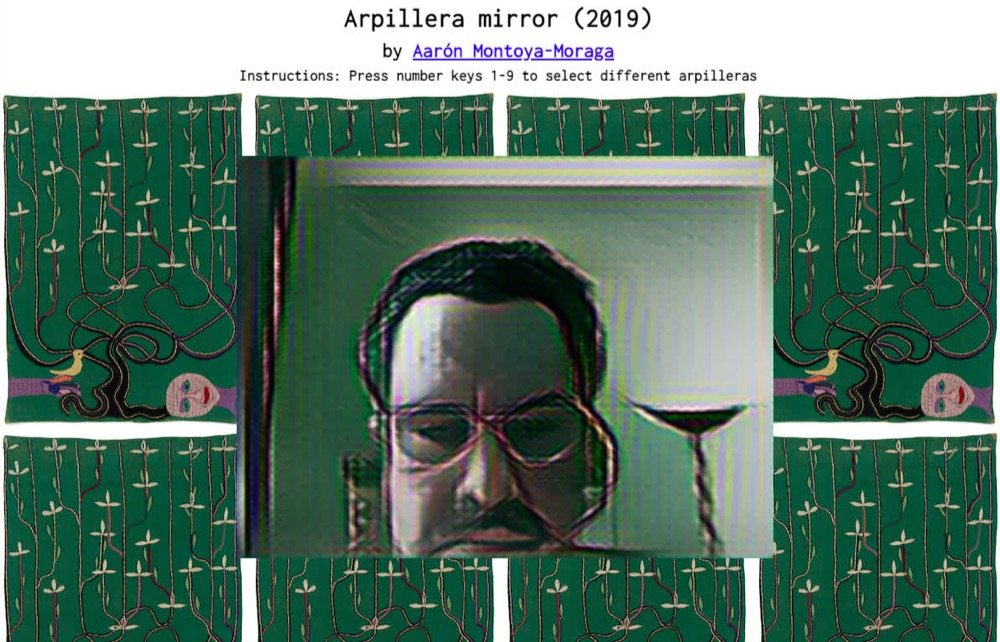
\includegraphics[width=0.75\linewidth,height=0.35\textheight,keepaspectratio]{images/arpillera-mirror.jpg}
  \caption{Arpillera Mirror, 2019}
  \caption*{Screen capture by myself}
  \label{fig:arpillera-mirror}
\end{figure}

 The source images for this project were obtained from the Violeta Parra museum's online collection. My original plan was to use this experiment to pitch two things to the Violeta Parra's museum: that they release their digital collection with permissive licenses, like the Digital Collections from the \acrfull{NYPL}, and to have a style transfer mirror with Violeta Parra's work included in their permanent collection. Since I haven't been able to visit Chile yet, this project is still unauthorized, and I haven't published the source code.

For people who are interested in the rich field of image generation with \acrshort{ML}, I highly recommend the book Making Pictures with Generative Adversarial Networks \cite{making-pictures-with-gans} by Casey Reas, published by Anteism, as of 2021 on its second edition. It’s an arts-first book that contextualizes the use of \acrshort{ML} algorithms for the creation of images, and uses the metaphor of these algorithms as being similar to the development of the camera. Artists don’t necessarily need to understand all the physics or mechanics behind a camera in order to make art with it, but it can definitely help to understand it too. I think that \acrshort{ML} is a revolutionary strategy for instrument-making and the arts, while also introducing new civic complexities, and in this thesis I have tried to follow the example of Reas' book, to introduce the technology and contextualize for a new generation of artists and instrument makers.

The last projects I want to mention in this section is the class Machine learning for physical computing \cite{repository-yining1023-machine-learning-for-physical-computing} written and taught in 2020 by software developer Yining Shi \cite{website-yining-shi} at \acrshort{NYU} \acrshort{ITP}. This class was the first time I saw a project building on top of the recently released library TensorFlow Lite for microcontrollers. This class inspired me to also use this library as a jumpstart for Tiny Trainable Instruments.

\chapter{Background and inspiration}

\section{Microcontrollers as alternative to computers}

When I joined MIT Media Lab in 2019, I made the decision to focus my efforts on hardware research, so I could make computational art devices, instead of software that needs to run on a laptop computer or a browser. This was fueled by the introduction of restrictive news by Apple, such as advising against the use of apps created by unregistered developers and discontinuing support for 32-bit apps, and by the ever-changing nature of the web, which makes my online artwork break often and need maintenance, and the need for additional corporate infrastructure to keep it online. In contrast I saw hardware as a space where I could deploy my ideas and keep them running without outside intervention.

I started my research by catching up with the newer developments by Teensy. The newer microcontrollers are faster and more powerful, and I used them to design and implement many small projects. I want to mention this personal project, a standalone audiobook I made with rotary encoders and a small screen for navigation, because it led me to include software for support of this same screen in the TinyTrainable library.

\begin{figure}[ht]
  \centering
  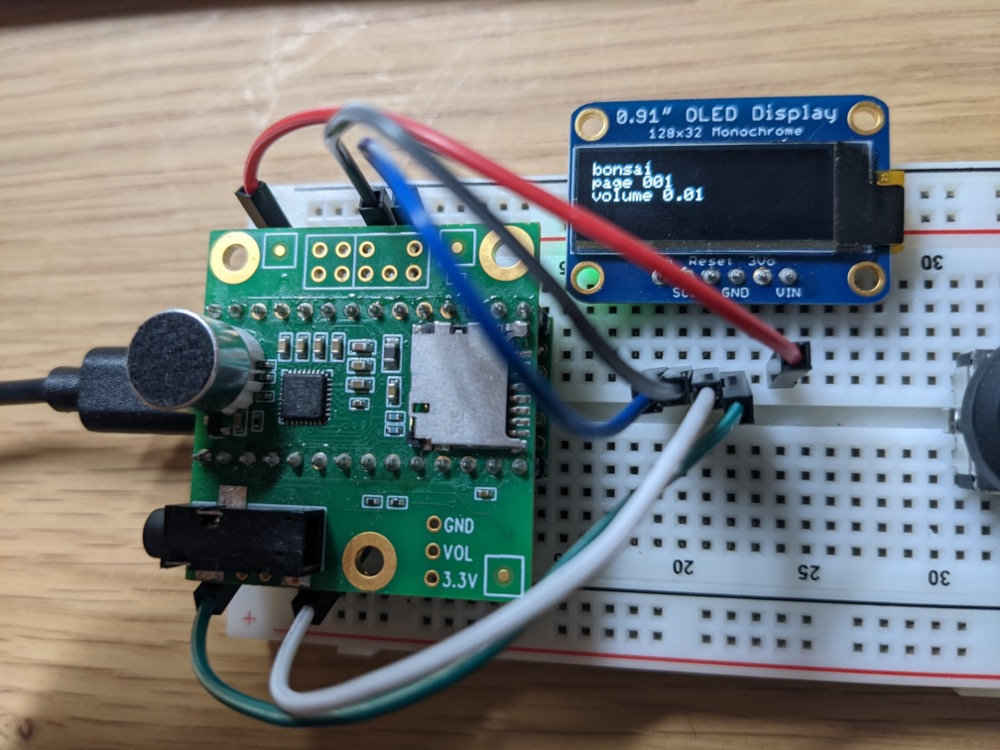
\includegraphics[width=0.75\linewidth,height=0.40\textheight,keepaspectratio]{images/bonsai.jpg}
  \caption{Audiobook made with Teensy}
  \caption*{Picture taken by myself}
  \label{fig:bonsai-audiobook}
\end{figure}

In parallel, I researched the evolution of the teaching of physical computing at \acrshort{NYU} \acrshort{ITP}, and I discovered that they stopped teaching with the now classic Arduino Uno, and have replaced it with the newer series of Arduino Nano microcontrollers, which have a smaller format and and operating voltage of 3.3V instead of 5V.

While browsing this series, I discovered the Arduino Nano 33 \acrshort{BLE} Sense that I based my thesis on. It comes with 9 embedded sensors, to measure and detect acceleration, movement, distance, color, plus a microphone. This is an amazing help for beginners, since a huge challenge when you are starting to build your own projects and learning electronics is reading datasheets to understand what sensors you can use with your microcontroller, how to wire them and calibrate them, and then what library supports it. This makes it easier and cheaper to prototype, and this made my work on my thesis easier, since I didn't have to include instructions for wiring sensors or calibrating them, and I could focus on \acrshort{ML} and the different outputs for arts.

\section{Coursework at MIT}

As part of the research that directly inspired this thesis, here is the coursework I took at MIT, and my notes about how they inform my theoretical and practical background for Tiny Trainable Instruments.

\begin{enumerate}
  \item Fall 2019, CMS.901 Current Debates in Media, by Professor Sasha Costanza-Chock
  \item Fall 2019, MAS.S65 Recreating The Past, by Professor Zach Lieberman
  \item Spring 2020, MAS.826 Sound: Past and Future, by Professor Tod Machover
  \item Spring 2020, MAS.712 Learning Creative Learning, by Professor Mitchel Resnick
\end{enumerate}

In the class Current Debates in Media, topics covered included fake news, surveillance, algorithmic bias, data colonialism, climate justice, algorithms of oppression, among others. For my final paper I wrote on the role of the media during the 2019 Chilean protests. This class directly inspired me to look for privacy-first \acrshort{ML}, and thinking about \acrshort{AI} in a critical way and not as clean safe automation, but as invisibilized labor, exploitation, and algorithmic bias and discrimination in the worst scenarios.

In the class Recreating the Past, I learned about media arts history, and I dived deep into the language C++ which I used for writing the TinyTrainable library, while working with the library openFrameworks, which is one of the most popular open source frameworks and communities for media arts.

In the class Sound: Past and Future, I learned more about the history of different computational advancements for sound, with a strong focus on projects at the MIT Media Lab's own research groups including Opera of the Future, Hyperinstruments, and Music, Mind, and Machine. This class introduced me to many projects and it helped me decide on making instruments for my thesis, using the latest technologies I could find, in this case, microcontrollers and \acrshort{ML}.

In the class Learning Creative Learning, I was introduced to the Lifelong Kindergarten's frameworks and ideas, including the 4 P's (projects, passion, peers, and play), and the design of Scratch as a home with low floor, wide walls, and high ceiling, which I highly recommend to follow up with  on Mitchel Resnick's book Lifelong Kindergarten \cite{lifelong-kindergarten}. This class gave me the push to write my software library with a community in mind, starting with the development of it. I made this happen by working with MIT undergrads Peter Tone and Maxwell Wang, who helped me with different aspects of research and development.

\subsection{TinyML Professional Certificate}

Apart from the MIT coursework, between November 2020 and March 2021 I completed the online Tiny Machine Learning Professional Certificate by Harvard University at the platform edx \cite{website-edx-harvardx-tinymlx-professional-certificate}. It is a series of three courses, where they teach responsible \acrshort{AI} strategies, theoretical \acrshort{ML}, and applied tiny \acrshort{ML} with the Arduino Nano 33 BLE Sense microcontroller, with a focus on industrial applications.

The academic team behind this certificate released the companion Harvard tinyMLx Arduino library \cite{repository-tinymlx-arduino-library}, which is based on the vanilla Arduino TensorFlowLite for microcontrollers. Through the example of this library, I learned how to build my own library for this thesis.

During this coursework I researched other libraries for machine learning, and discovered the Arduino \acrshort{k-NN} library \cite{repository-arduino-knn}. I included this library as a dependency on my thesis because it allows on-device data capture and model training. This allows for the data never leaving the device, and to enhance privacy, which is one of the driving concepts of this project.

\section{Research projects at MIT}

Another aspect of my research that I want to highlight is other research projects I worked on while at the MIT Media Lab, because they follow my same interests and passions, and I hope they help inform the process behind my thesis.

\subsection{SiguesAhi}

SiguesAhi \cite{website-library-siguesahi} (from the Spanish "Are you still there?") is an instrument to detect when oppressive institutions have ceased to exist. It is achieved with microcontrollers with internet connectivity.  I built it using a microcontroller from the same series and format but different architecture and capabilities, the Arduino Nano 33 IoT.

\begin{figure}[ht]
  \centering
  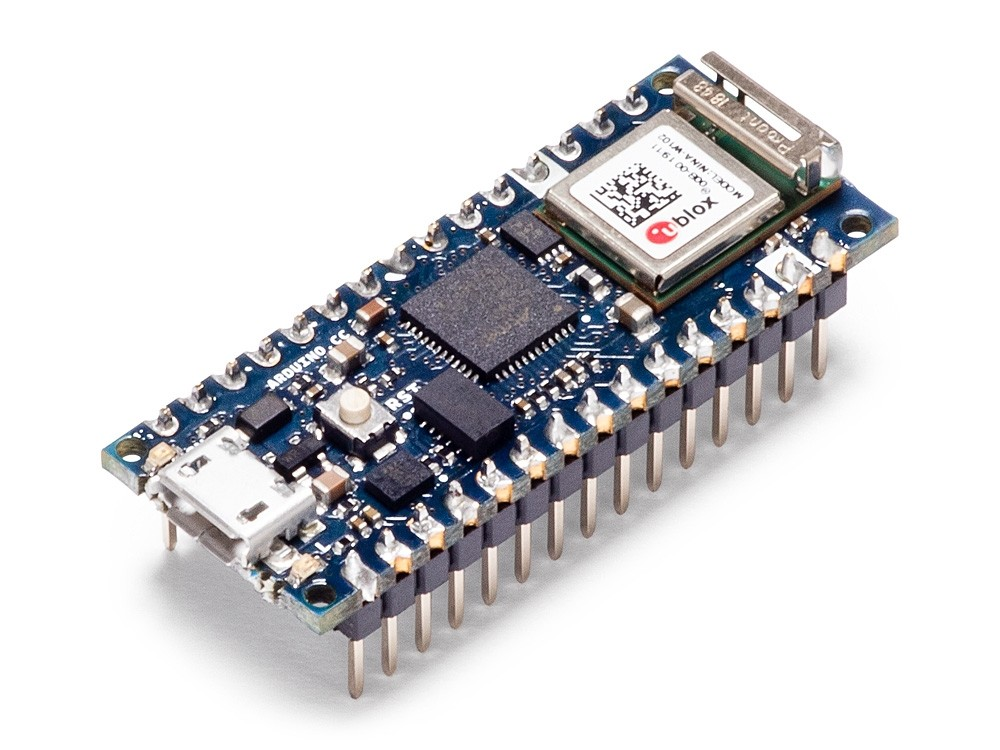
\includegraphics[width=0.75\linewidth,height=0.20\textheight,keepaspectratio]{images/arduino-nano-33-iot-with-headers.jpg}
  \caption{Arduino Nano 33 IoT with headers}
  \caption*{Retrieved from \cite{website-arduino-nano-33-iot-with-headers}}
  \label{}
\end{figure}

SiguesAhi's functionality is accomplished by connecting the microcontroller to the internet, and making it periodically download the first paragraph of the institution's Wikipedia article. Then the microcontroller checks if the first sentence is written in either present or past tense, and determines the existence of the institution. In the examples published in the alpha version of the software library \cite{website-library-siguesahi}, I am monitoring the National Rifle Association, which sadly still exists. 

\begin{figure}[ht]
  \centering
  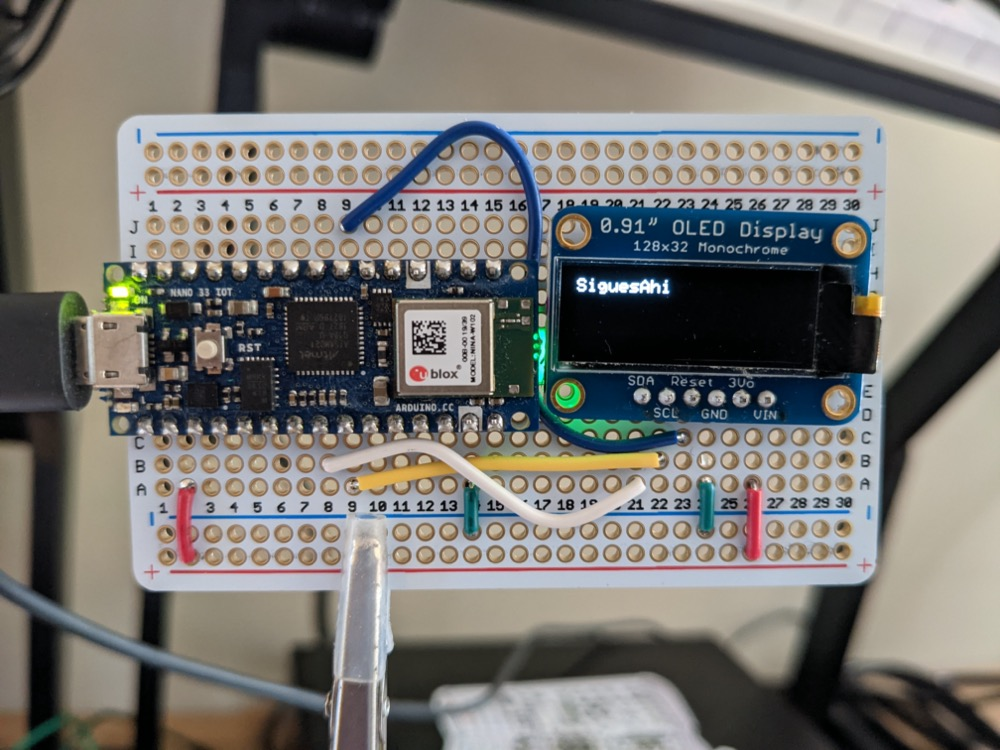
\includegraphics[width=0.75\linewidth,height=0.25\textheight,keepaspectratio]{images/siguesahi.jpg}
  \caption{SiguesAhi project}
  \caption*{Picture by myself}
  \label{fig:siguesahi}
\end{figure}

As a feature, I am adding support for Wikipedia articles in different languages, with the hope that people can use this library to make their own instruments to track the downfall of oppressive institutions wherever they are. I am building one for myself to track the existence of the current Chilean Constitution, written in 1980 by the military dictatorship.

SiguesAhi has been developed in parallel to Tiny Trainable Instruments, and has been possible thanks to the techniques and strategies I have learned about instrument making and publishing software libraries for arts.

\subsection{Open Drawing Machine}

The Open Drawing Machine \cite{website-open-drawing-machine} is a collaborative project with Gaurav Patekar for the research group Future Sketches at the MIT Media Lab. It is a low cost open source machine, consisting of an Arduino microcontroller and hardware for drawing computationally.

\begin{figure}[ht]
  \centering
  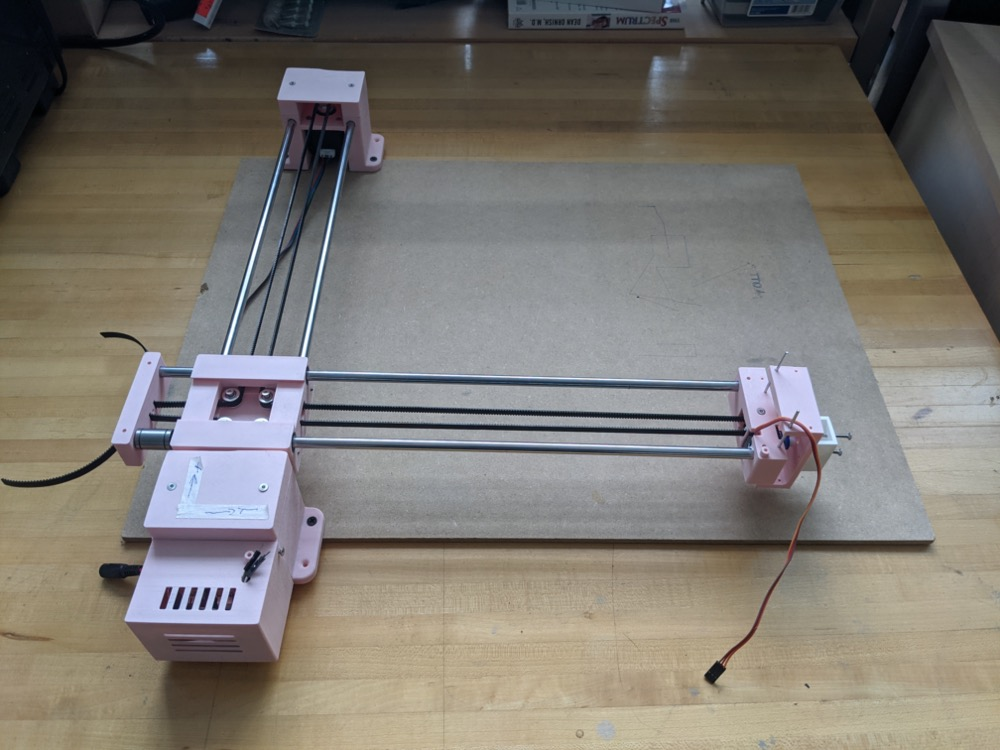
\includegraphics[width=0.75\linewidth,height=0.25\textheight,keepaspectratio]{images/open-drawing-machine.jpg}
  \caption{Open Drawing Machine project}
  \caption*{Picture by myself}
  \label{fig:open-drawing-machine}
\end{figure}

Gaurav Patekar designed and 3D-printed the hardware, and I packaged our code and published a library add-on for openFrameworks. Currently the Open Drawing Machine can receive drawing commands from a computer through a serial port, and the next step of this project is being able to receive commands from other computers through networks and the internet.

\subsection{Introduction to networks for artists}

Introduction to networks for artists \cite{website-intro-to-computer-networks-for-artists} is a series of tutorials for beginners, to learn how to set up their own networks and collaborate remotely in peer-to-peer ways for making art, featuring several open source software tools for arts. This project is inspired by the amazing research on remote collaboration, body sensors, peer-to-peer protocols, by movement artist and programmer Lisa Jamhoury \cite{website-lisa-jamhoury}, including the app Kinectron \cite{website-repository-kinectron}, to which I am a contributor.

\begin{figure}[ht]
  \centering
  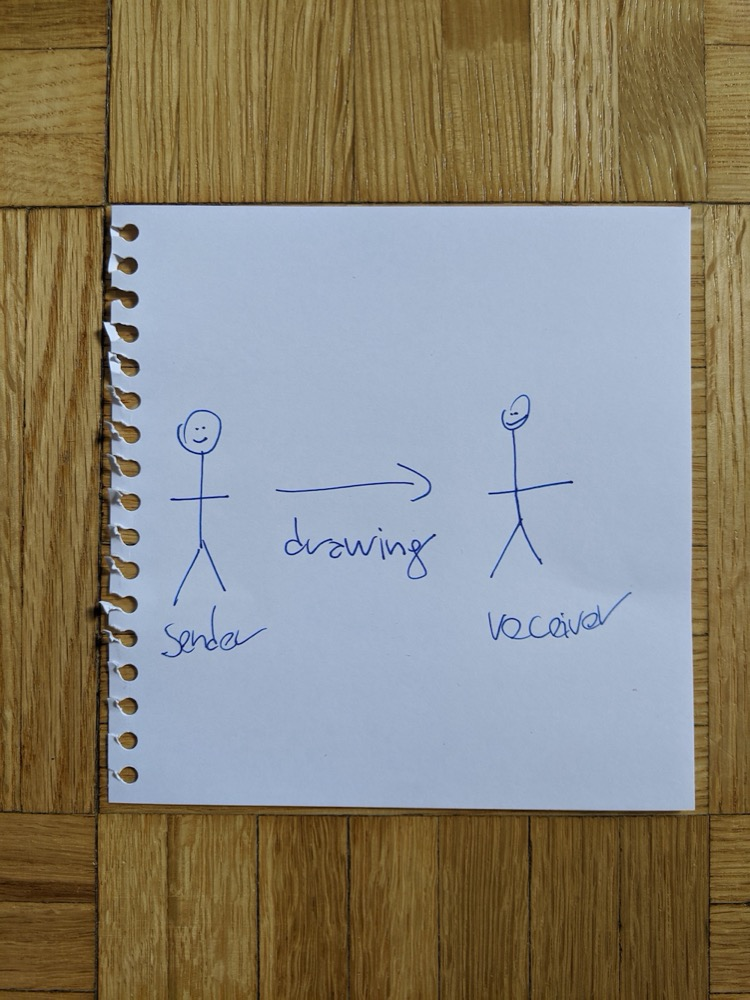
\includegraphics[width=0.75\linewidth,height=0.35\textheight,keepaspectratio]{images/intro-to-computer-networks-for-artists.jpg}
  \caption{Introduction to computer networks for artists project}
  \caption*{Picture by myself}
  \label{fig:intro-to-computer-networks-for-artists}
\end{figure}

\section{Computational media arts instruments}

A big concentration of my research at the MIT Media Lab is computational media arts instruments. I define them as devices that convert the data from an input like human gesture, to process and output different media (audio, video, text, light, etc), using digital operations.

Nowadays artists have access to a rich ecosystem of computers, operating systems and software for making art, and it is common for them to rely on their personal computer for making all of their art, on the go, wherever they are. In the 1990s, musicians stopped having to rely on analog hardware for recording and mixing, and broadly embraced digital technology, with a huge reduction in costs and maintenance.

In this section of my thesis I will share my research on companies making some of my favorite recent computational media arts instruments, with a strong focus on the ones that can be programmed, and that promote open source hardware or software. Many of these instruments often sit at my desk for inspiration, or I spend hours playing with them for my art and learning from them and the communities around them.

The tables \ref{table:media-arts-instruments-technical} and \ref{table:media-arts-instruments-influence} are respectively summaries of techniques and influences of the instruments that I reference in this section.

\begin{table}[ht]
    \centering
    \begin{tabular}{ | l |  l | l | l | l |}
        \hline
        \textbf{Company} & \textbf{Instrument} & \textbf{Year} & \textbf{Basis} & \textbf{Software} \\
        \hline
        Bastl Instruments   & Illuminati    & 2019  & MCU       & None                \\
        \hline
        Bastl Instruments   & Kastle Drum   & 2020  & MCU       & Arduino, C++        \\
        \hline
        Bastl Instruments   & Kastle v1.5   & 2017  & MCU       & Arduino, C++        \\
        \hline
        Bastl Instruments   & OMSynth       & 2016  & IC        & None                \\
        \hline
        Bastl Instruments   & microGranny 2 & 2016  & MCU       & Arduino, C++        \\
        \hline
        Bastl Instruments   & Servo         & 2016  & MCU       & Arduino, C          \\
        \hline
        Critter \& Guitari  & Organelle     & 2016  & Linux     & Pure Data           \\
        \hline
        Critter \& Guitari  & EYESY         & 2020  & Linux     & Python, Pygame      \\
        \hline
        monome              & aleph         & 2013  & Linux     & C                   \\
        \hline
        monome              & norns         & 2018  & Linux     & Lua, SuperCollider  \\
        \hline
        Shbobo              & Shnth         & 2013  & MCU       & Shlisp              \\
        \hline
        Shbobo              & Shtar         & 2017  & MCU       & Shlisp              \\
        \hline
    \end{tabular}
    \caption{Technical details of media arts instruments}
    \label{table:media-arts-instruments-technical}
\end{table}{}

\begin{table}[ht]
    \centering
    \begin{tabular}{ | l |  l | l |}
        \hline
        \textbf{Company}    & \textbf{Instrument} & \textbf{Influence}              \\
        \hline
        Bastl Instruments   & Illuminati    & Output with LEDs                      \\
        \hline
        Bastl Instruments   & Kastle series & Use of breadboard and jumper wires    \\
        \hline
        Bastl Instruments   & OMSynth       & Distribution as tutorials + parts kit \\
        \hline
        Bastl Instruments   & microGranny 2 & Arduino as basis for instrument       \\
        \hline
        Bastl Instruments   & Servo         & Output with servo motor               \\
        \hline
        Critter \& Guitari  & Organelle     & Scriptable audio computer             \\
        \hline
        Critter \& Guitari  & ETC, EYESY    & Scriptable visuals computer, screen output\\
        \hline
        monome              & aleph, norns  & Scriptable audio computer            \\
        \hline
        Shbobo              & Shnth, Shtar  & Multiple input sensors, scripting     \\
        \hline
    \end{tabular}
    \caption{Influence of media arts instruments}
    \label{table:media-arts-instruments-influence}
\end{table}{}

\subsection{Bastl Instruments}

Bastl Instruments is a Czech company of multimedia instruments, which has had a huge impact and influence on my research and practice. When I first started researching the Eurorack format some years ago, I visited the shop Control in Brooklyn, NY, and some modules by Bastl stood out to me, because of their wooden panels and interaction with classic physical computing educational materials, such as motors and solenoids, which was an inspiration for me to include servo motors as an output option in the Tiny Trainable Instruments.

\begin{figure}[ht]
  \centering
  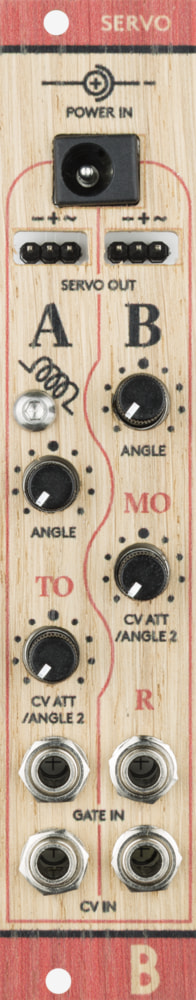
\includegraphics[width=0.75\linewidth,height=0.25\textheight,keepaspectratio]{images/bastl-servo.jpg}
  \caption{Bastl Instruments Servo module}
  \caption*{Retrieved from \cite{website-bastl-instruments-current}}
  \label{fig:bastl-servo}
\end{figure}

Another inspiration comes from their microGranny 2 granular sampler which is made with an Atmega microcontroller and its firmware is open source and available as a repository on their GitHub account \cite{github-bastl-instruments}, along with many other of their instruments.

\begin{figure}[ht]
  \centering
  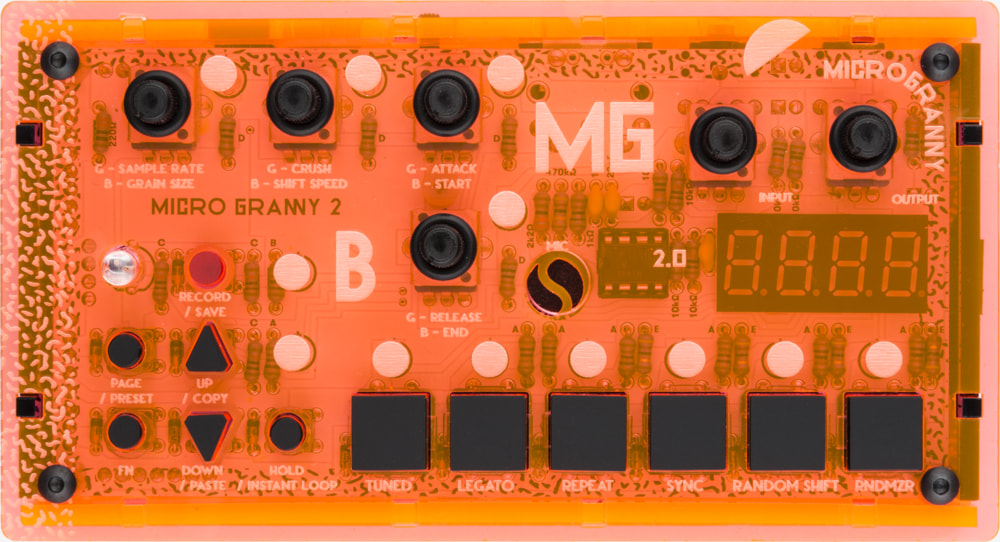
\includegraphics[width=0.75\linewidth,height=0.25\textheight,keepaspectratio]{images/bastl-microgranny-2.jpg}
  \caption{Bastl Instruments microGranny 2}
  \caption*{Retrieved from \cite{website-bastl-instruments-current}}
  \label{fig:bastl-microgranny-2}
\end{figure}

Their Kastle synthesizers are also based on microcontrollers, and feature a patchbay for making connections with jumper wires, the same used for prototyping in electronic breadboards. This influenced me to build the Tiny Trainable Instruments with breadboards and jumper wires, instead of custom \acrshortpl{PCB}.

\begin{figure}[ht]
  \centering
  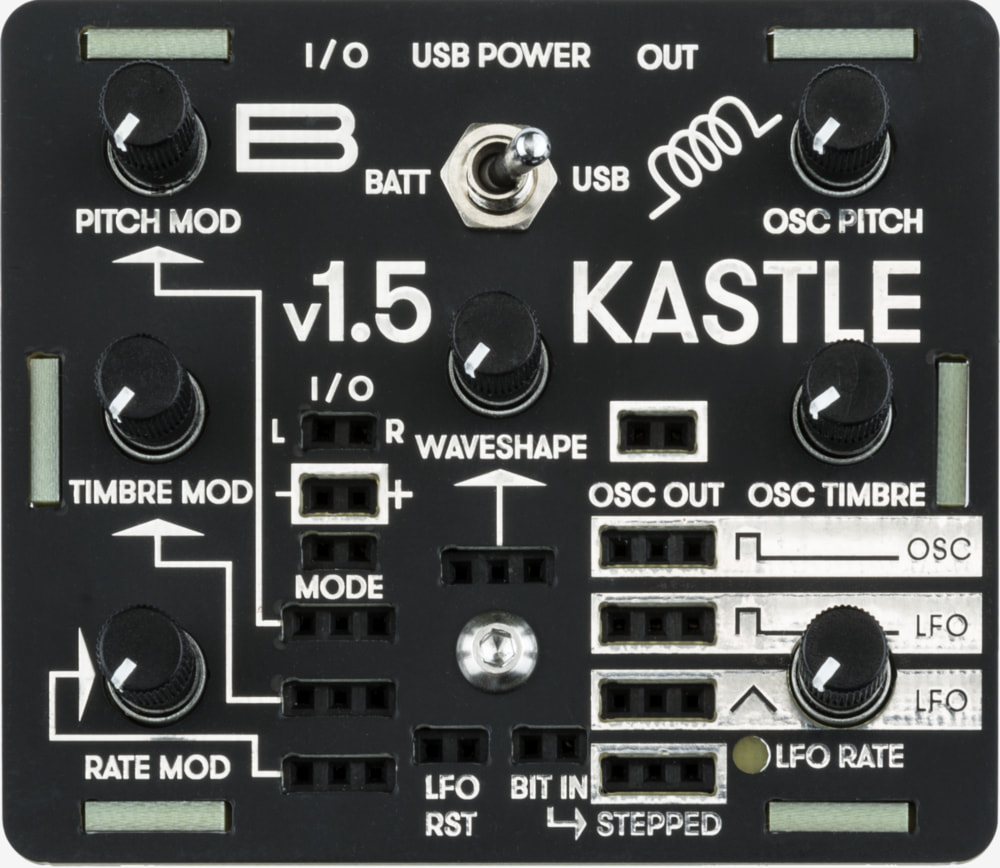
\includegraphics[width=0.75\linewidth,height=0.25\textheight,keepaspectratio]{images/bastl-kastle-v15.jpg}
  \caption{Bastl Instruments Kastle v1.5}
  \caption*{Retrieved from \cite{website-bastl-instruments-current}}
  \label{fig:bastl-kastle-v15}
\end{figure}

Also, the Kastle synths are forgiving instruments, their inputs and outputs are robust enough to allow for mistakes in connections, in an electrical and mechanical way, which I think is perfect for safe experimentation. It would be a bummer if the instrument was easy to break, or if it demanded a huge effort in understanding electronics for using it. 

As of writing, two different units are in production, both retailing for around 100.00 USD: the Kastle v1.5 melodic / drone synthesizer, and the Kastle Drum, for rhythm. The only difference between these synthesizers is the firmware and the labels on the faceplate. The community is encouraged to write new firmware to modify their behavior. 

\begin{figure}[ht]
  \centering
  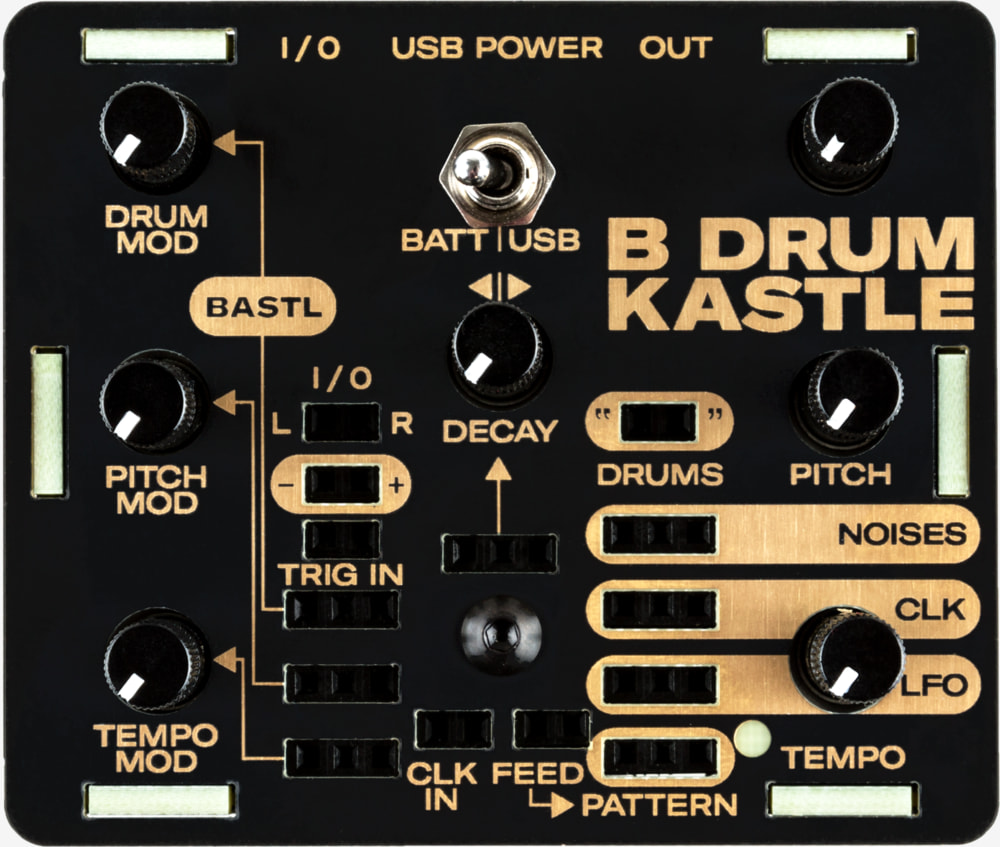
\includegraphics[width=0.75\linewidth,height=0.25\textheight,keepaspectratio]{images/bastl-kastle-drum.jpg}
  \caption{Bastl Instruments Kastle Drum}
  \caption*{Retrieved from \cite{website-bastl-instruments-current}}
  \label{fig:bastl-kastle-drum}
\end{figure}

Another instrument I want to highlight is the Illuminati, currently discontinued, a device that uses different inputs (audio, control voltage, \acrshort{MIDI} messages) to control the light intensity of connected USB lamps, which influenced the conception of Tiny Trainable Instruments as multimedia arts instruments, not only focusing on audio and music, but also printed text, light, and screen output.

\begin{figure}[ht]
  \centering
  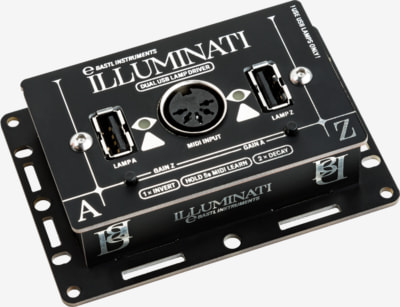
\includegraphics[width=0.75\linewidth,height=0.25\textheight,keepaspectratio]{images/bastl-illuminati.jpg}
  \caption{Bastl Instruments Illuminati}
  \caption*{Retrieved from \cite{website-bastl-instruments-current}}
  \label{fig:bastl-illuminati}
\end{figure}

The final instrument from this company that I want to highlight is the OMSynth, one of Bastl Instruments' many collaborations with Casper Electronics. This device is an educational and maker circuit development tool for creating synthesizers. It includes basic fundamental blocks, such as battery power, audio input and output, potentiometers for attenuating and boosting signals, and a suite of parts kits for building devices including sequencers, oscillators, and samplers, on the included breadboard. Its release as a kit was also a direct influence on the kits I designed for the workshops I taught with the Tiny Trainable Instruments.

\begin{figure}[ht]
  \centering
  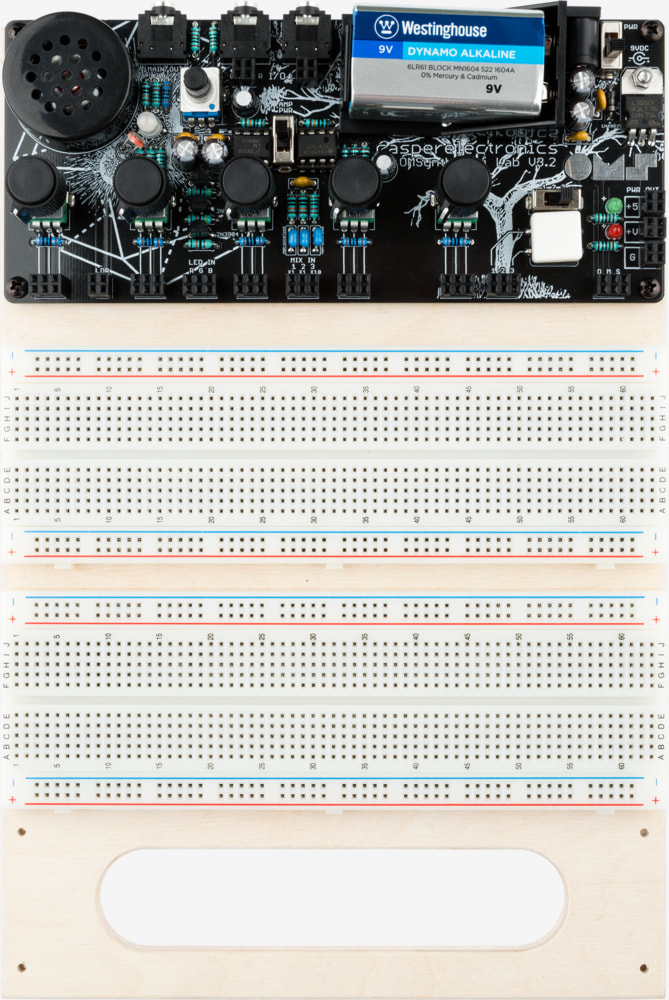
\includegraphics[width=0.75\linewidth,height=0.25\textheight,keepaspectratio]{images/bastl-omsynth.jpg}
  \caption{Bastl Instruments OMSynth}
  \caption*{Retrieved from \cite{website-bastl-instruments-current}}
  \label{fig:bastl-omsynth}
\end{figure}

Many Bastl standalone instruments are 200.00 USD or less, which is a huge contrast to the 1960s, when a Moog analog system II cost 6,200.00 USD, which was enough to buy a small house \cite{analog-days}. Also, many of their instruments are sold as kits for building and soldering them yourself, for the cheaper cost and the added educational aspect of having hands-on experience.

\subsection{Critter \& Guitari}

Critter \& Guitari is an American company based in Brooklyn, NY, which has released several computational microcontroller-based audiovisual instruments, from which my favorite is the currently discontinued Kaleidoloop. It is a sampler with an internal speaker and an included microphone, that allows you to record and playback audio. The instrument features two knobs for controlling the volume and playback rate of audio loops from your recordings. I really admire its portability, in terms of its size, weight, and being battery-powered, encouraging the recording and making of music while walking or in the park. This was a major influence on the design of the Tiny Trainable Instruments; the materials I picked are intended for building standalone instruments that you can power with a USB power bank or a battery, so that you can take them for a walk too.

\begin{figure}[ht]
  \centering
  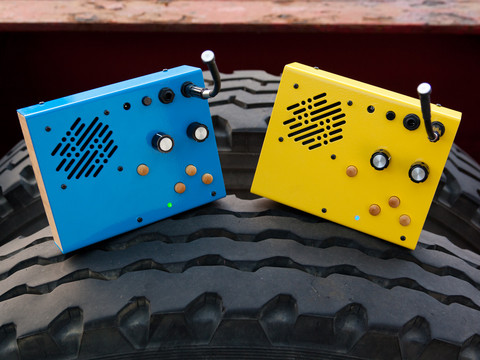
\includegraphics[width=0.75\linewidth,height=0.25\textheight,keepaspectratio]{images/critter-and-guitari-kaleidoloop.jpg}
  \caption{Critter \& Guitari Kaleidoloop}
  \caption*{Retrieved from \cite{website-critter-and-guitari-kaleidoloop}}
  \label{fig:critter-and-guitari-kaleidoloop}
\end{figure}

In 2015, Critter \& Guitari released the Organelle, a sound computer running the Linux operating system, and the \acrfull{Pd} software for programming patches that reacts to the computer's interface (knobs, encoders, keys), and then generates sound. It is currently on its second iteration, called Organelle M, with added features, such as an embedded speaker and microphone.

\begin{figure}[ht]
  \centering
  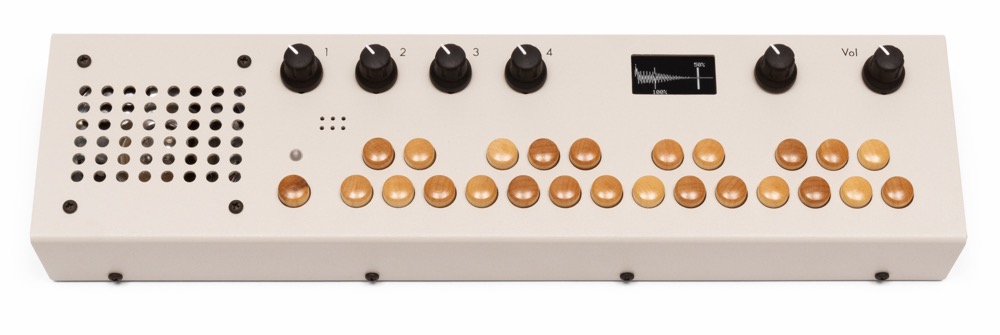
\includegraphics[width=0.75\linewidth,height=0.25\textheight,keepaspectratio]{images/critter-and-guitari-organelle-m.jpg}
  \caption{Critter \& Guitari Organelle M}
  \caption*{Retrieved from \cite{website-critter-and-guitari-current}}
  \label{fig:critter-and-guitari-organelle-m}
\end{figure}

Since the sound generation is made with the software \acrshort{Pd}, you can achieve the same sonic results on an Organelle or on your personal computer. Despite this, I am convinced that the Organelle is a revolutionary instrument,  because it allows artists to use computation in a single-purpose and stable device for their sound, in heavy contrast with the over-bloated personal computers we use from activities ranging from watching movies to paying taxes, and which constantly require updates and maintenance. The Organelle also replaces the keyboard and mouse in computers with an interface tailored for contemporary music production, including a musical keyboard for playing notes, knobs and encoders for changing parameters, and a screen for navigating menus.

The final aspects I want to celebrate about the Organelle are its ever growing capabilities, and the community behind it: Critter \& Guitari regularly publishes new \acrshort{Pd} patches, and the community also organizes in forums and repositories to share their creations. You don't need to be a programmer to enjoy the Organelle, you can download and use the new presets without ever having to open a code editor.

After the release of the Organelle, this company released the ETC visuals computer. It also runs the Linux operating system, and it uses the pygame Python library for generating graphics which can then be projected on a screen.  The ETC was discontinued and replaced with the EYESY, with upgrades such as a new mode for running openFrameworks.

\begin{figure}[ht]
  \centering
  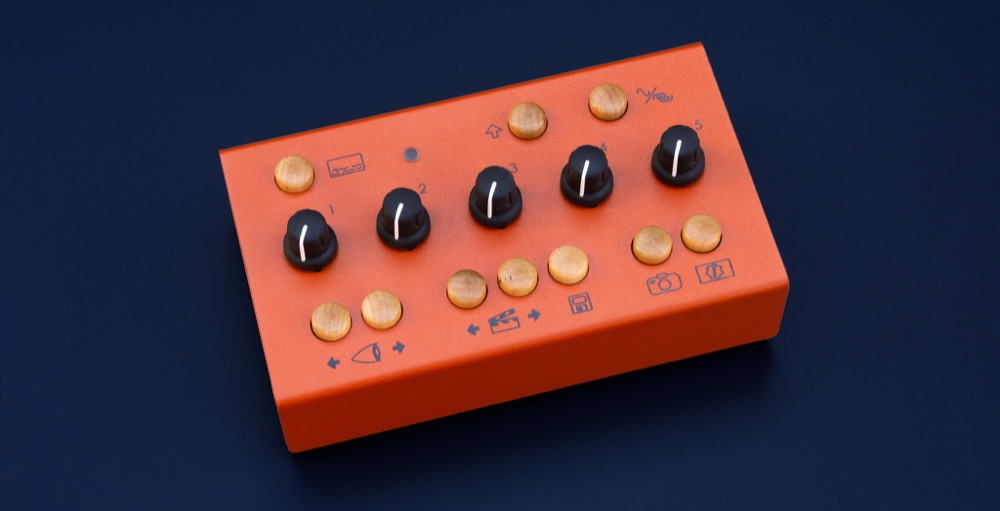
\includegraphics[width=0.75\linewidth,height=0.25\textheight,keepaspectratio]{images/critter-and-guitari-eyesy.jpg}
  \caption{Critter \& Guitari EYESY}
  \caption*{Retrieved from \cite{website-critter-and-guitari-current}}
  \label{fig:critter-and-guitari-eyesy}
\end{figure}

The current lineup of the Organelle and EYESY computers for arts make Critter \& Guitari a pioneering company in the creation of scriptable instruments that run open source software and foster communities around them. Tiny Trainable Instruments is heavily indebted to the work of this company, trying to promote scripting for microcontrollers for a new generation of artists.

\subsection{monome}

monome \cite{website-monome-current} is an American company based in upstate New York. Their first instrument was the grid, still in production. In its current iteration, it consists of 128 backlit silicone keys distributed in 8 rows and 16 columns. It has a USB port, through which it can be connected to all sorts of devices, including computers and Eurorack modules.

\begin{figure}[ht]
  \centering
  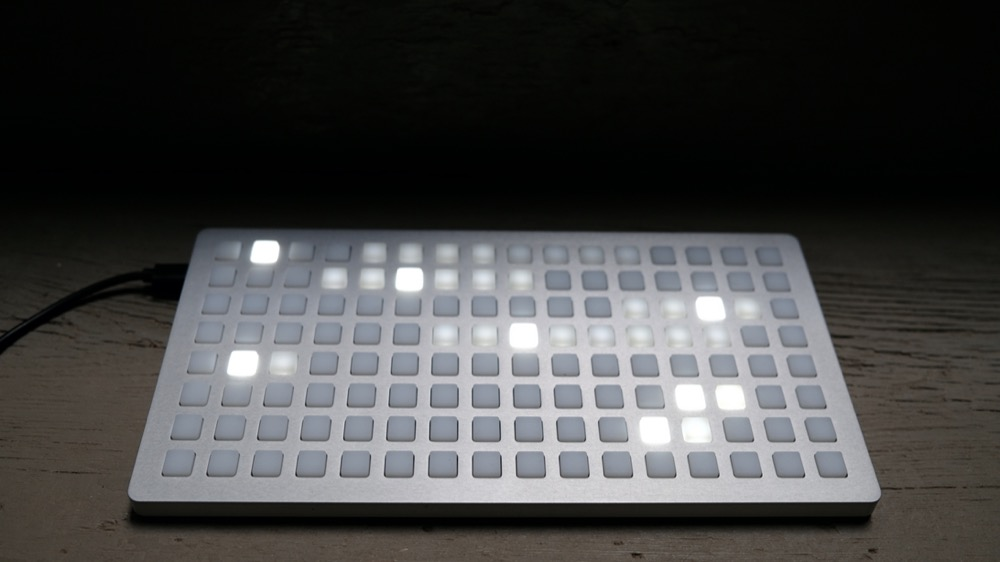
\includegraphics[width=0.75\linewidth,height=0.25\textheight,keepaspectratio]{images/monome-grid.jpg}
  \caption{monome grid}
  \caption*{Retrieved from \cite{website-monome-current}}
  \label{fig:monome-grid}
\end{figure}

The monome website features extensive tutorials for learning how to interface the grid with many popular open source hardware and software systems, including Arduino, Processing, \acrshort{Pd}, SuperCollider, Python, and Node.js. Over the years I have learned many important lessons about instrument making, software for arts, and live performance with my grid, and I am including what I learned on this thesis project.

Through the grid, I learned about the other instruments by monome, and I want to highlight the open source sound computers they have released, starting with the now-discontinued aleph.

\begin{figure}[ht]
  \centering
  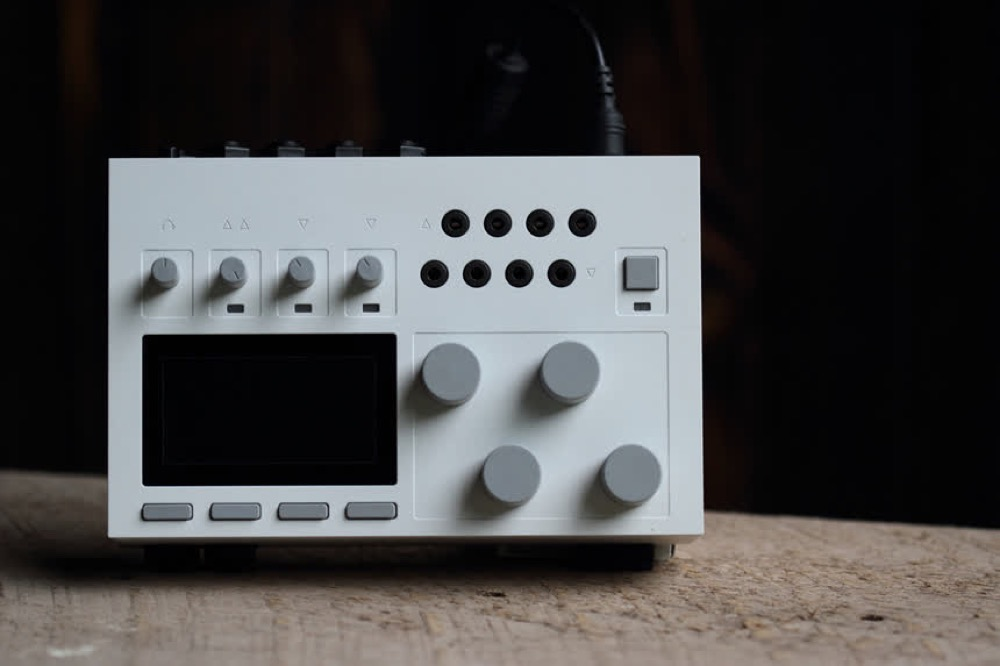
\includegraphics[width=0.75\linewidth,height=0.25\textheight,keepaspectratio]{images/monome-aleph.jpg}
  \caption{monome aleph}
  \caption*{Retrieved from \cite{website-monome-current}}
  \label{fig:monome-aleph}
\end{figure}

The aleph had a focus on community building by releasing the technical documentation and guides for enthusiasts to write and share their own extensions of the software, written in the C programming language. Even though monome only made 100 units of the aleph, it directly influenced their next sound computer, norns, currently available both as an instrument and a \acrshort{DIY} shield for the Raspberry Pi computer.

\begin{figure}[ht]
  \centering
  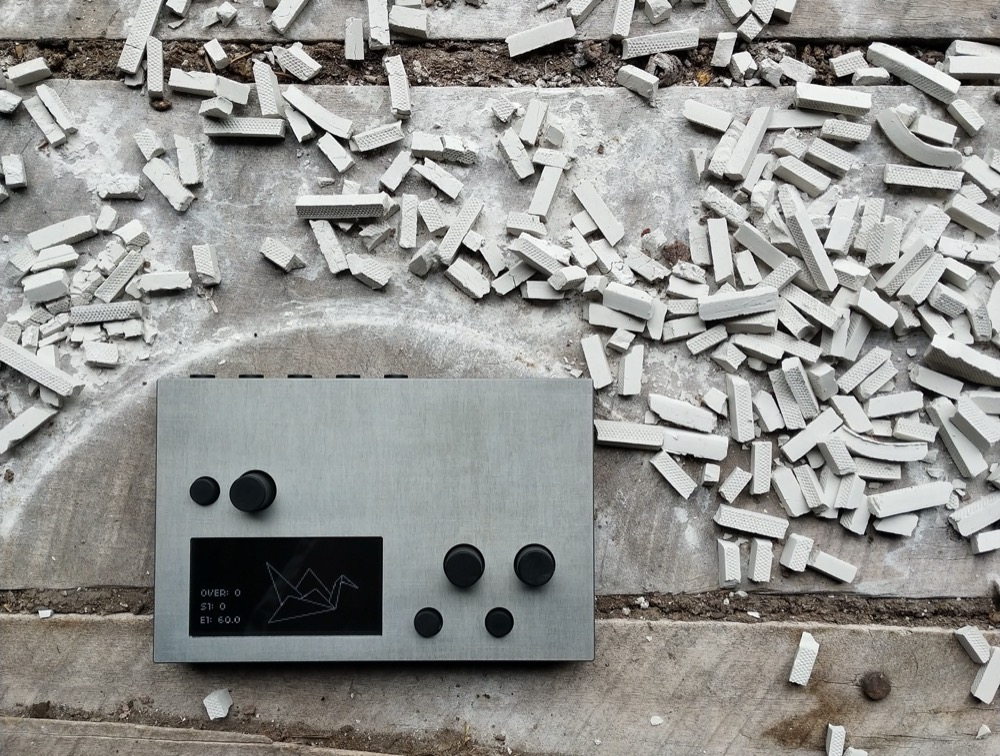
\includegraphics[width=0.75\linewidth,height=0.25\textheight,keepaspectratio]{images/monome-norns.jpg}
  \caption{monome norns}
  \caption*{Retrieved from \cite{website-monome-current}}
  \label{fig:monome-norns}
\end{figure}

The norns runs the Linux operating system, uses SuperCollider for sound generation, and runs Lua scripts for other tasks, such as reading the data from the buttons and encoders, displaying visuals on the screen, and sharing variables with the sound engine. Users are encouraged to write their own software in these two languages, and there is a strong community, both at monome's forum \url{https://norns.community/} and at the norns wiki \url{https://norns.community/}.

\subsection{Shbobo}

In my first semester at MIT, I was introduced by classmate Will Freudenheim \cite{website-will-freudenheim}  to the Shbobo Shnth synthesizer by Peter Blasser. The Shnth is a microcontroller-based scriptable instrument, with multiple input sensors, including flex sensors,  a microphone, and capacitive skin proximity.

\begin{figure}[ht]
  \centering
  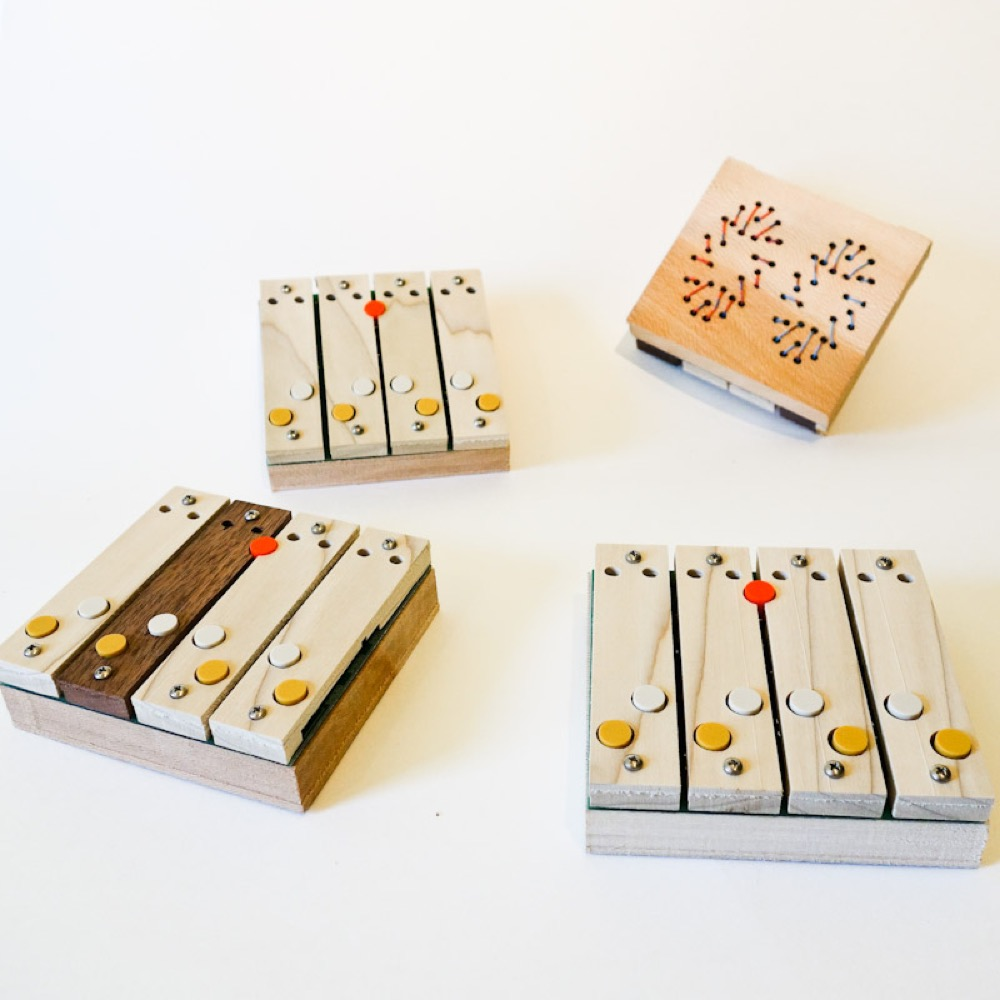
\includegraphics[width=0.75\linewidth,height=0.25\textheight,keepaspectratio]{images/shbobo-shnth.jpg}
  \caption{Shbobo Shnth}
  \caption*{Retrieved from \cite{website-shbobo-current}}
  \label{fig:shbobo-shnth}
\end{figure}

Peter Blasser is an instrument maker, dedicated to \gls{synthesynthesis}, the synthesis of synthesizers \cite{blasser2015stores}. Peter has created several companies of musical instruments, each one of them with different features and philosophies. The most famous one is Ciat-Lonbarde, which use banana cables to make connections between their jacks, for sharing audio and control signals. Another companies include Tocante, with a line of solar-powered touch-based instruments, and Ieaskul F. Mobenthey, a line of Eurorack modules.

For this thesis I want to focus on the company Shbobo, a digital collection of instruments based on microcontrollers, which is made up of the already mentioned Shnth, and the Shtar, a 17-fret string instrument.

\begin{figure}[ht]
  \centering
    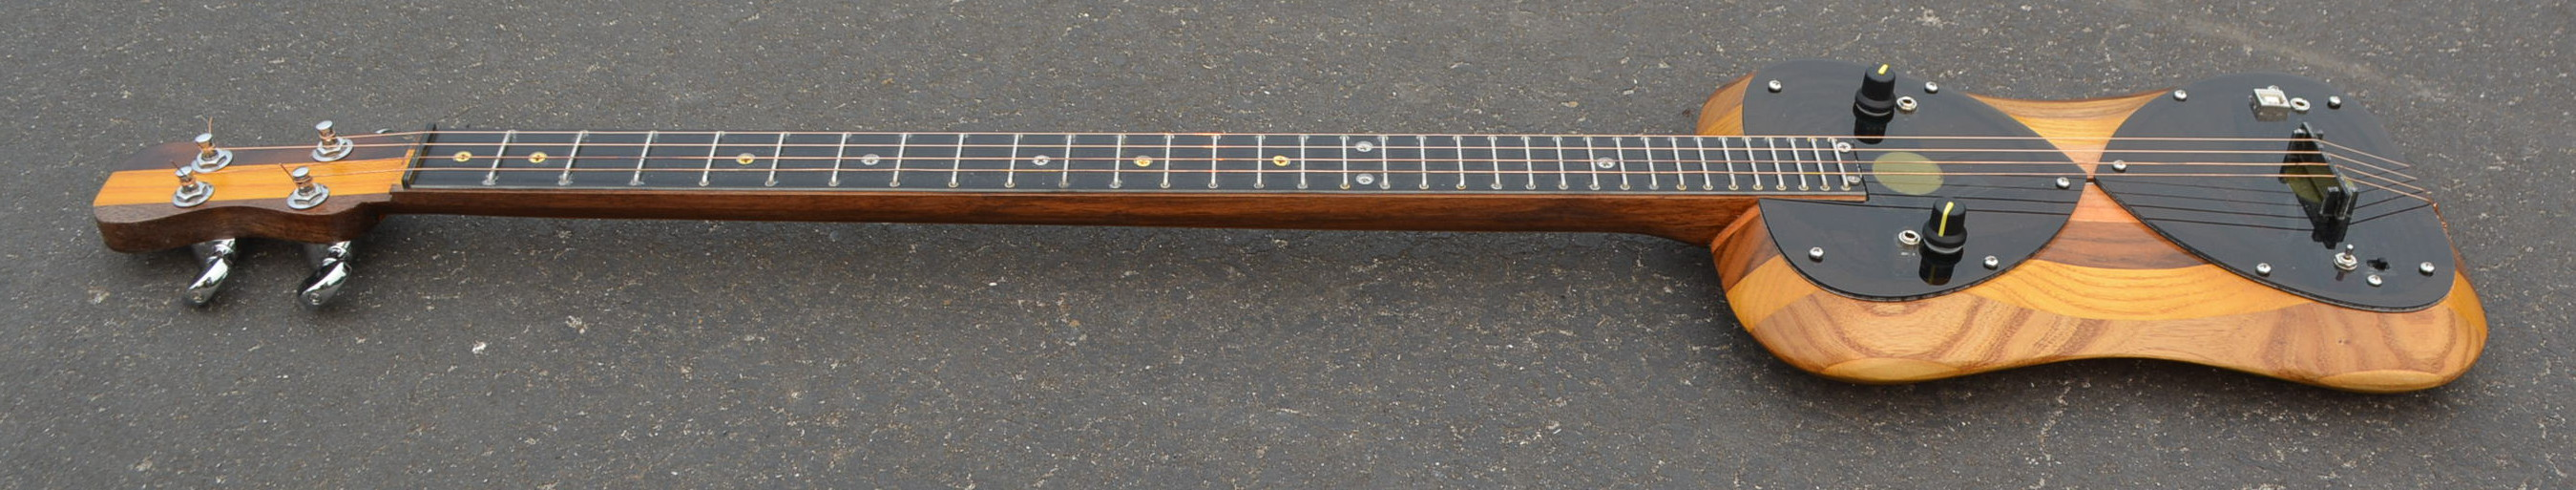
\includegraphics[width=0.75\linewidth,height=0.25\textheight,keepaspectratio]{images/shbobo-shtar.jpg}
  \caption{Shbobo Shtar}
  \caption*{Retrieved from \cite{website-shbobo-current}}
  \label{fig:shbobo-shtar}
\end{figure}

Both the Shnth and the Shtar can be programmed using an open source language called Shlisp, available at \url{https://github.com/pblasser/shbobo}. The Shlisp language allows the use of different sensors on the instruments to control different oscillators, filters, and effects, and interactions between the sound engine and the instrument interface. Just like all of the instruments by Peter Blasser, the Shbobo instruments don't follow classical Western musical conceptions of notes and scales, but rather follow the approach of pioneers such as Don Buchla, by making their own language for describing the instruments' behavior and sounds.

They promote computer-centric approaches to making sound, such as the use of integers and metaphors of finite state machines, and also allow for different ways of playing and sensing, such as the use of antennas for detecting hand distance, a microphone for detecting speech and whistling, and wooden bars with piezos for detecting pressure.

\section{Education}

This thesis is also inspired by the work of the research group Lifelong Kindergarten at the MIT Media Lab, led by professor Mitchel Resnick. In the book with the same title, he builds on Seymour Papert’s work and proposes that educational projects should have “Low floor, wide walls, high ceilings.” Additionaly, that learners thrive when they engage in the 4 Ps: “Projects, passion, peers, and play.”

In terms of projects, this thesis includes the release of a software library, so that people can make the software their own, and spin off their own projects. It is also open source so that people can learn from my mistakes and also \gls{fork} to adapt to their needs.

In terms of passion, this thesis is a contribution to the ecosystem of instrument makers, so that other people can enjoy my same passion, of making art with computation.

In terms of peers, I have been lucky to have been supported by the MIT UROP office and MIT Media Lab, and had the opportunity to work with MIT undergrad researchers Peter Tone and Maxwell Wang. Also, this project was taught in collaborative workshops where people could discuss their ideas with their peers.

In terms of play, this thesis project is not about correct answers, or even excellent classification with \acrshort{ML}, it's all about finding innovative ways to interact with multimedia material, celebrate the small victories and the big glitches, and iterate over and over again.

\section{Digital rights}


So far I have felt comfortable doing scraping in private, for academic or artistic purposes, but not for more public or commercial outlets. For Tiny Trainable Instruments, I was worried about including web scraping techniques, because I didn't want to infringe any copyrights or be involved in litigation.

Because of my concerns, I reached out to the Technology Law Clinic \cite{website-boston-university-technology-law-clinic} at Boston University's School of Law. My request was for them to assess the potential civil and criminal liabilities if I conducted web scraping on Youtube.com, in order to to train my machine learning algorithms. I also inquired about the legal implications of publishing my databases, my trained models, and related tutoria for encouraging other people to also do web scraping.

The Technology Law Clinic gave me a breakdown of the legal risks associated with web scraping, and they confirmed with me that I could be in violation of three different laws: the \acrfull{CFAA}, the \acrfull{DMCA}, and the Copyright Act. This confirmation cemented my decision of using the Arduino microcontroller as a source for my data, so that all my databases would be homemade and fully original. I hope my contributions in how to capture data, parse it, and how to use it to build your own databases is also helpful to others.

I am no expert on digital or human rights at all, but I am convinced that it's a human right to not be surveilled, and I hope this thesis helps to illustrate different strategies I have learned while at MIT. During my research and my class with Sasha Costanza-Chock, I studied or became aware of different efforts in programming for activism, including the Guardian Project by the Electronic Frontier Foundation, which made me decide to include privacy and consent as key topics on this project.

Since \acrshort{ML} algorithms need data to be trained on, and corporations and governments are hungry about gathering our data, it is of critical importance for this decade for people to be aware of the pitfalls and dangers of algorithmic bias and surveillance, and I think the techniques, documentation, and proposals I make for building custom databases for this project, help in the educational efforts for society's safe practices around their data.

I am constantly in awe of the work by countless activists and researchers, including Joy Buolamwini, Timnit Gebru, Deborah Raji, Chelsea Manning, Edward Snowden, and countless others who have spoken truth to power.

\section{Opera of the Future research projects}

During the development of this thesis, I have been fortunate to collaborate on different capacities with other thesis projects by classmates at the Opera of the Future research group, which has directly inspired my work.

\subsection{Squishies, by Hannah Lienhard}

Squishies is Hannah Lienhard's Master's thesis, and consists of novel squishable interfaces for musical expression. We shared discussions about low-level sound design, code reusability, sound art education, and digital instruments. We were part of a Master's thesis working group, facilitated by Roya Moussapour with two other Media Lab classmates, where we workshopped drafts of our thesis. This practice and feedback has been critical in shaping the language and discourse of this thesis document.

\subsection{Fluid Music, by Charles Holbrow}

Fluid Music is Charles Holbrow's PhD thesis. It is a software framework for music composition and production. The design of the interface, documentation, and scope of Charles' thesis were a direct influence on the documentation and API coding style of this project. I was fortunate to collaborate with Charles, by testing the software library, discussing documentation design, and participating in one of his workshops teaching with Fluid Music, which in turn inspired me to include my own workshop for user feedback and release of this project.

\chapter{Background and inspiration}

\epigraph{It has to start somewhere \\ it has to start sometime \\ what better place than here? \\ what better time than now?}{Guerrilla Radio \\ Rage Against the Machine, 1999}

\section{Microcontrollers as alternative to computers}

When I joined MIT Media Lab in 2019, I made the decision of focusing my efforts hardware research, so I could make computational art devices, instead of software that needs to run on a laptop computer or a browser. This was fueled by the introduction of restrictive news by Apple, such as advising against the use of apps created by unregistered developers and discontinuing support for 32 bit apps, and by the ever-changing nature of the web, which makes my online artwork break often and need maintenance, and the need for additional corporate infrastructure to keep it online. In contrast I saw hardware as a space where I could deploy my ideas and keep them runing without outside intervention.

I started my research by catching up with the newer developments by Teensy. The newer ones are faster and more powerful, and I usedm to design and implement many small projects. I want to mention this personal project, a standalone audiobook I made with rotary encoders and a small screen for navigation, because it led me to add of support of this same screen on the TinyTrainable library.

\begin{figure}[ht]
  \centering
  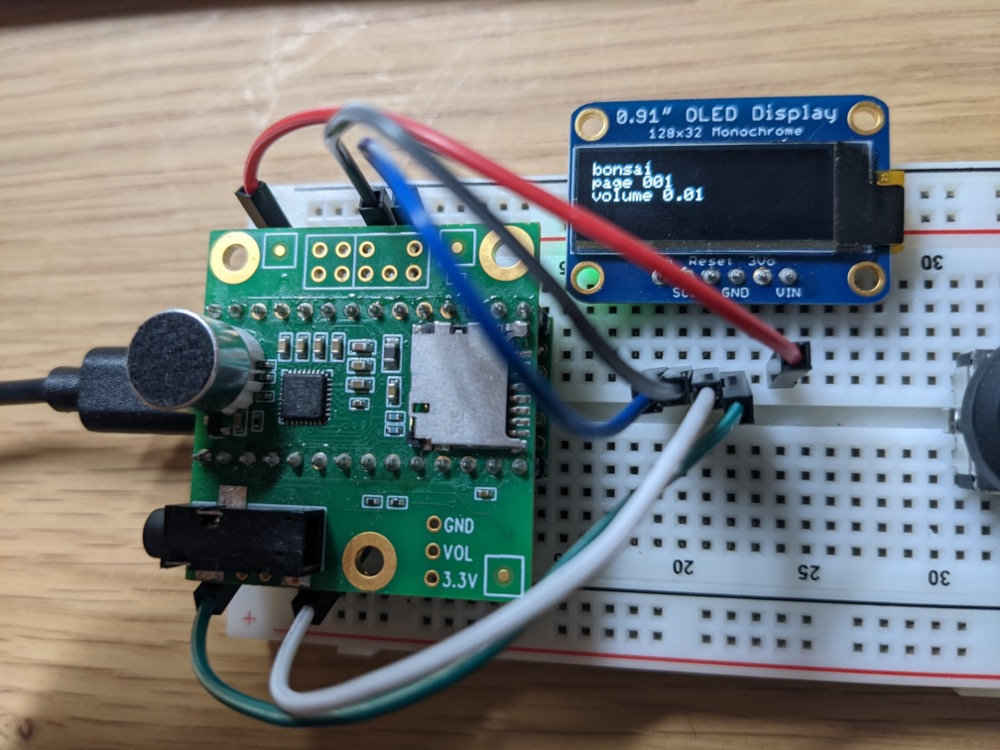
\includegraphics[width=0.75\linewidth,height=0.40\textheight,keepaspectratio]{images/bonsai.jpg}
  \caption{Audiobook made with Teensy}
  \caption*{Picture taken by myself}
  \label{fig:bonsai-audiobook}
\end{figure}

In parallel, I researched the evolution of the teaching of physical computing at \acrshort{NYU} \acrshort{ITP}, and I discovered that they stopped teaching with the now classic Arduino Uno, and have replaced it with the newer series of Arduino Nano microcontrollers, which have a smaller format and and operating voltage of 3.3V instead of 5V.

While browsing this series, I discovered the Arduino Nano 33 \acrshort{BLE} Sense that I based my thesis now. It comes with 9 emedded sensors, to measure and detect acceleration, movement, distance, color, and a microphone. This is an amazing help for beginners, since a huge challenge when you are starting to build your own projects and learning electronics, is reading datasheets to understand what sensors you can use with your microcontroller, how to wire them and callibrate them, and then what library supports it. This makes it easier and cheaper to prototype, and this made my work on my thesis easier, since I didn't have to include instructions for wiring sensors or callibrating them, and I could focus on \acrshort{ML} and the different outputs for arts.

\section{Coursework at MIT}

As part of the research that directly inspired this thesis, here is the coursework I took, and my notes about how they inform my theoretical and practical background for Tiny trainable instruments.

\begin{enumerate}
  \item Fall 2019, CMS.901 Current Debates in Media, by professor Sasha Costanza-Chock
  \item Fall 2019, MAS.S65 Recreating The Past, by professor Zach Lieberman
  \item Spring 2020, MAS.826 Sound: Past and Future, by Tod Machover
  \item Spring 2020, MAS.712 Learning Creative Learning, by professor Mitchel Resnick
\end{enumerate}

In the class Current Debates in Media, topics covered included fake news, surveillance, algorithmic bias, data colonialism, climate justice, algorithms of oppression, among others. For my final paper I wrote on the role of the media during the 2019 Chilean protests. This class directly inspired me to look for privacy-first \acrshort{ML}, and thinking about \acrshort{AI} in a critical way and not as clean safe automation, but as invisibilized labor, exploitation, and algorithmic bias and discrimination in the worst scenarios.

In the class Recreating the Past, I learned about media arts history, and I dived deep in the language C++ which I used for writing the TinyTrainable library, while working with the library openFrameworks, which is one of the most popular open source frameworks and communities for media arts.

In the class Sound: Past and Future, I learned more about the history of different computational advancements for sound, with a strong focus on projects at MIT Media Lab's own research groups including Opera of the Future, Hyperinstruments, and Music, Mind, and Machine. This class introduced me to many projects and it helped me decide on making instruments for my thesis, using the latest technologies I could find, in this case, microcontrollers and \acrshort{ML}.

In the class Learning Creative Learning, I was introduced to the Lifelong Kindergarten's frameworks and ideas, including the 4 P's (peers, projects, passion, and play), and the design of Scratch as a home with low floor, wide walls, and high ceiling, which I highly recommend to check on Mitchel Resnick's book Lifelong Kindergarten. This class gave me the push to write a library with a community in mind, starting with the development of it, which happened because I had the pleasure of working with MIT undergrads Peter Tone and Maxwell Wang, who helped me with different aspects of research and development.

\section{Research projects at MIT}

Some other projects I created during this master's include:

\begin{enumerate}
  \item SiguesAhi: an instrument to detect when oppressive institutions have ceased to exist. It is achieved with microcontrollers with Internet connectivity.
  \item Open Drawing Machine, with Gaurav Patekar: an open source low cost programmable drawing machine
  \item Introduction to networks for artists: a series of tutorials for beginners, to learn how to set up their own networks and collaborate in peer-to-peer ways for making art.
\end{enumerate}

SiguesAhi is a sibling project to Tiny trainable instruments. It is based on a microcontroller from the same series and format but different architecture and capabilities, the Arduino Nano 33 IoT.

\begin{figure}[ht]
  \centering
  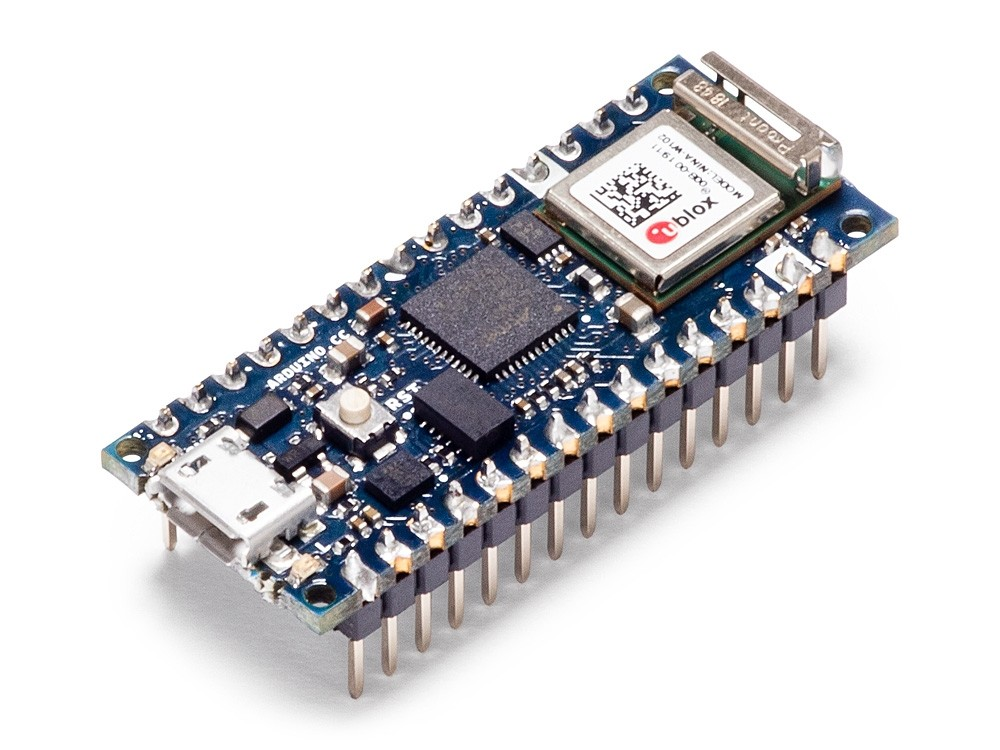
\includegraphics[width=0.75\linewidth,height=0.25\textheight,keepaspectratio]{images/arduino-nano-33-iot-with-headers.jpg}
  \caption{Arduino Nano 33 IoT with headers}
  \caption*{Retrieved from \cite{website-arduino-nano-33-iot-with-headers}}
  \label{}
\end{figure}

For this project, I am writing a library for making digital instruments that can detect if institutions still exist. This is accomplished by connecting the microcontroller to the internet, and making it ping the Wikipedia website with a certain periodicity, in order to download and check the first sentence of the first paragraph of the entry. As an example of the library, I am using the National Rifle Association, which sadly still exists.

\begin{figure}[ht]
  \centering
  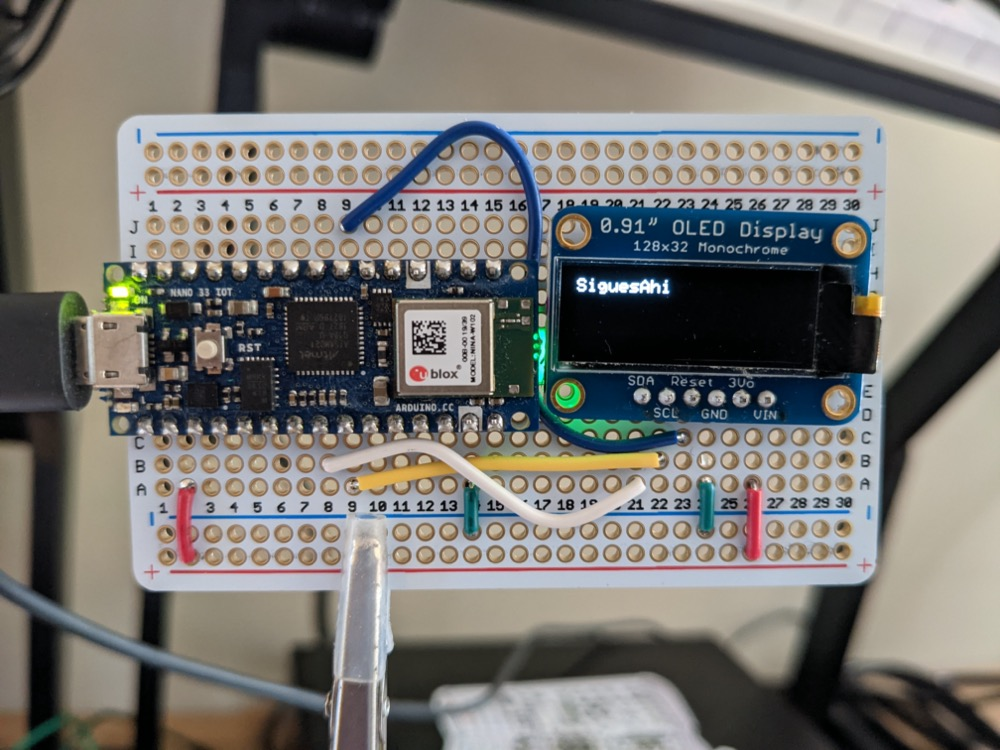
\includegraphics[width=0.75\linewidth,height=0.25\textheight,keepaspectratio]{images/siguesahi.jpg}
  \caption{SiguesAhi project}
  \caption*{Picture by myself}
  \label{fig:siguesahi}
\end{figure}

The \cite[Open Drawing Machine]{website-open-drawing-machine} is a collaborative project with Gaurav Patekar for the research group Future Sketches at MIT Media Lab. It is a low cost open source machine, consisting of an Arduino microcontroller and hardware for drawing computationally. We have done the research together, Gaurav designed and 3D printed the hardware, and I have packaged the results as a still unfinished openFrameworks addon.

\begin{figure}[ht]
  \centering
  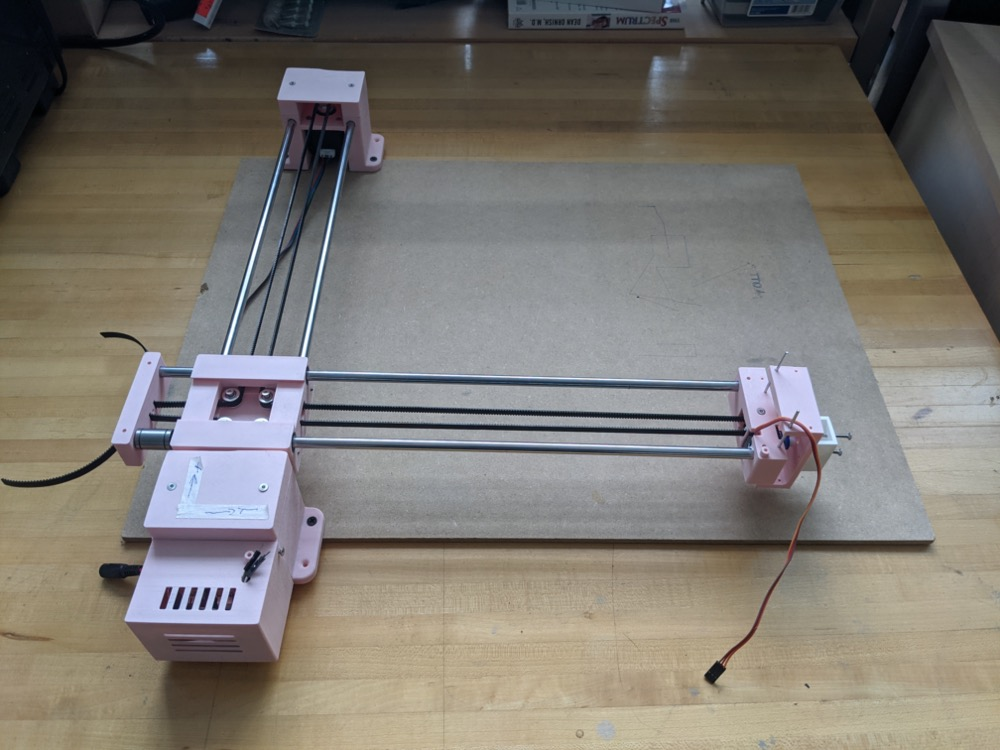
\includegraphics[width=0.75\linewidth,height=0.25\textheight,keepaspectratio]{images/open-drawing-machine.jpg}
  \caption{Open Drawing Machine project}
  \caption*{Picture by myself}
  \label{fig:open-drawing-machine}
\end{figure}

Currently the Open Drawing Machine can receive drawing commands from a computer through a serial port, and the next step of this project is being able to receive commands from other computers through networks and the internet. This comes from the last project I will mention that I worked on while at MIT Media Lab, which is Introduction to computer networks for artists \cite{website-intro-to-computer-networks-for-artists}, a collection of tutorials for remote peer-to-peer collaboration between artists. This project is inspired by the amazing research on remote collaboration, sensors, peer-to-peer protocols, by friend Lisa Jamhoury, including the app Kinectron

\begin{figure}[ht]
  \centering
  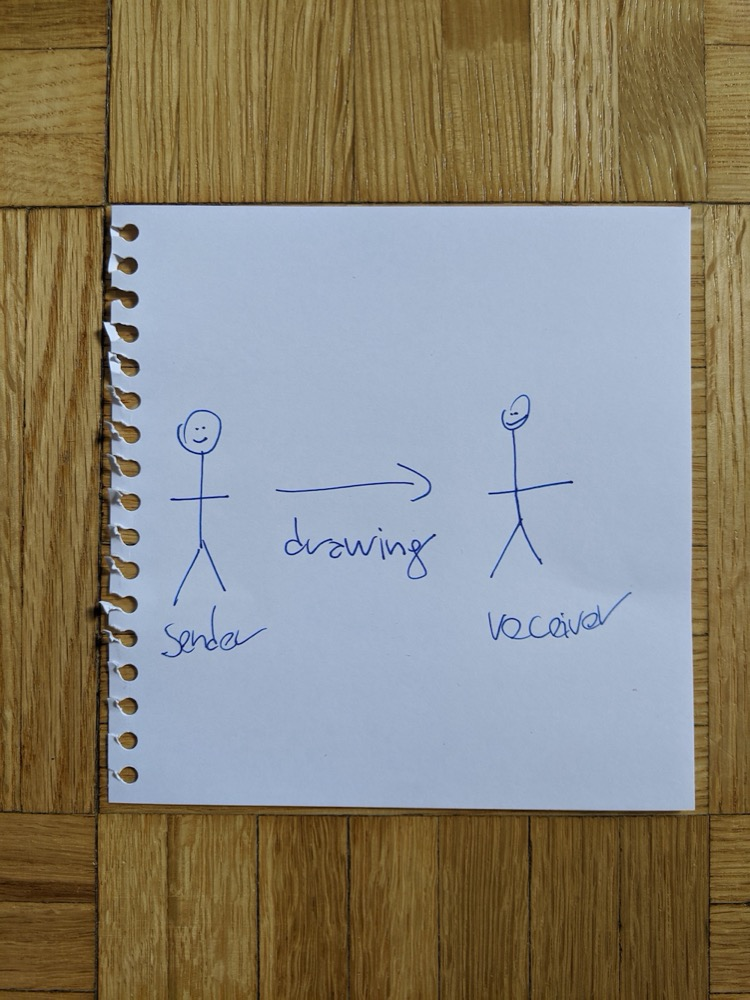
\includegraphics[width=0.75\linewidth,height=0.25\textheight,keepaspectratio]{images/intro-to-computer-networks-for-artists.jpg}
  \caption{Introduction to computer networks for artists project}
  \caption*{Picture by myself}
  \label{fig:intro-to-computer-networks-for-artists}
\end{figure}

\section{Companies making computational media arts instruments}

There is a rich ecosystem of personal computers, operating systems and software for making art, and it is common nowadays for artists to rely on their computer for making all of their art, on the go, wherever they are. Until recently, musicians relied on very expensive hardware for recording on tape, and now they can do it on their computers.

In music I have seen hybrid setups, where people do most of their work on the computer, but also rely on other specialized hardware, such as effects, mixers, and even all sorts of analog devices to give a different flavor to the recordings.

In particular, here I will highlight some media arts instruments that have inspired my research, because of their use and promotion of open source software and hardware, scripting capabilities, and other design considerations. These instruments often sit at my desk for inspiration, or I spend hours playing with them for my art and learning from them and the communities around them.

The tables \ref{table:media-arts-instruments-technical} and \ref{table:media-arts-instruments-influence} are respectively summaries of techniques and influences of the instruments that I reference in this section.

\begin{table}[ht]
    \centering
    \begin{tabular}{ | l |  l | l | l | l |}
        \hline
        Company             & Instrument    & Year  & Basis & Software            \\
        \hline
        Bastl Instruments   & Illuminati    & 2019  & MCU       & None                \\
        Bastl Instruments   & Kastle Drum   & 2020  & MCU       & Arduino, C++        \\
        Bastl Instruments   & Kastle v1.5   & 2017  & MCU       & Arduino, C++        \\
        Bastl Instruments   & OMSynth       & 2016  & IC        & None                \\
        Bastl Instruments   & microGranny 2 & 2016  & MCU       & Arduino, C++        \\
        Bastl Instruments   & Servo         & 2016  & MCU       & Arduino, C          \\
        Critter \& Guitari  & Organelle     & 2016  & Linux     & Pure Data           \\
        Critter \& Guitari  & EYESY         & 2020  & Linux     & Python, Pygame      \\
        monome              & aleph         & 2013  & Linux     & C                   \\
        monome              & norns         & 2018  & Linux     & Lua, SuperCollider  \\
        Shbobo              & Shnth         & 2013  & MCU       & Shlisp              \\
        Shbobo              & Shtar         & 2017  & MCU       & Shlisp              \\
        \hline
    \end{tabular}
    \caption{Technical details of media arts instruments}
    \label{table:media-arts-instruments-technical}
\end{table}{}

\begin{table}[ht]
    \centering
    \begin{tabular}{ | l |  l | l |}
        \hline
        Company             & Instrument    & Influence                             \\
        \hline
        Bastl Instruments   & Illuminati    & Output with LEDs                      \\
        Bastl Instruments   & Kastle series & Use of breadboard and jumper wires    \\
        Bastl Instruments   & OMSynth       & Distribution as tutorials + parts kit \\
        Bastl Instruments   & microGranny 2 & Arduino as basis for instrument       \\
        Bastl Instruments   & Servo         & Output with servo motor               \\
        Critter \& Guitari  & Organelle     & Computer for sound                    \\
        Critter \& Guitari  & EYESY         & Output with screen                    \\
        monome              & aleph, norns  & Computer for sound                    \\
        Shbobo              & Shnth, Shtar  & Input with multiple gestures          \\
        \hline
    \end{tabular}
    \caption{Influence of media arts instruments}
    \label{table:media-arts-instruments-influence}
\end{table}{}

\subsection{Bastl Instruments}

Bastl Instruments is a Czech company of multimedia instruments, which has had a huge impact and influence on my research and practice. When I first started researching the Eurorack format some years ago, I visited the shop Control in Brooklyn NY, and some modules by Bastl stood out to me, because of their wooden panels and interaction with classic physical computing educational materials, such as motors and solenoids, which was an inspiration for me to include support for servo motors in Tiny trainable instruments.

\begin{figure}[ht]
  \centering
  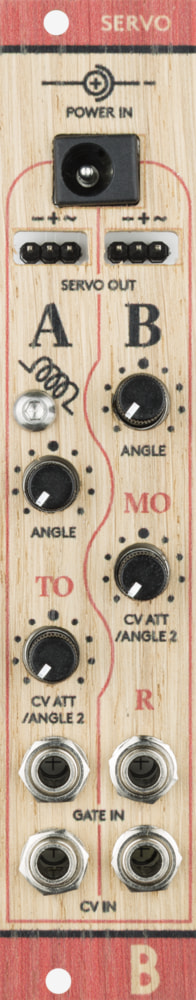
\includegraphics[width=0.75\linewidth,height=0.25\textheight,keepaspectratio]{images/bastl-servo.jpg}
  \caption{Bastl Instruments Servo module}
  \caption*{Retrieved from \cite{website-bastl-instruments-current}}
  \label{fig:bastl-servo}
\end{figure}

Another inspiration comes from their microgranny 2 granular sampler which is made with an Atmega microcontroller and its firmware is open source and available as a repository on their GitHub account, along with many other of their instruments.

\begin{figure}[ht]
  \centering
  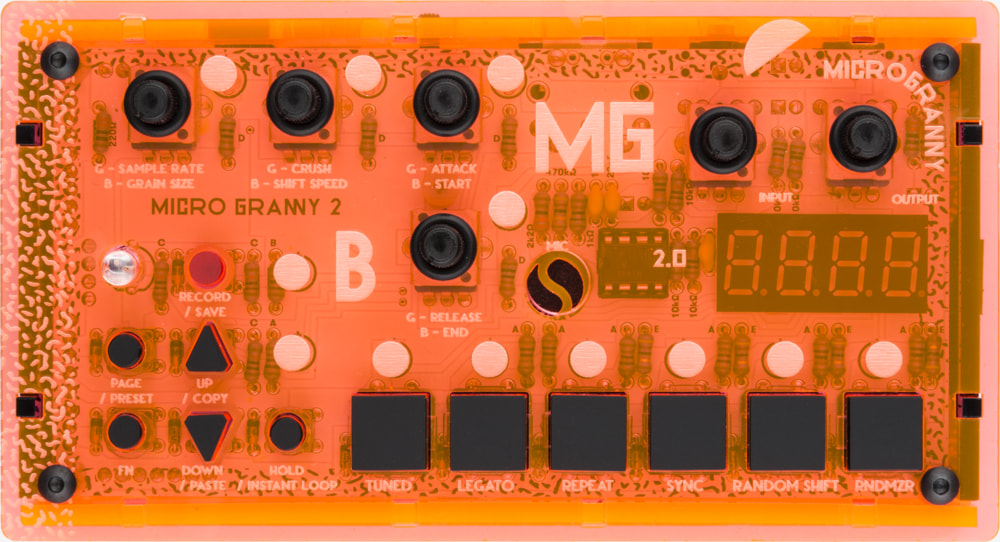
\includegraphics[width=0.75\linewidth,height=0.25\textheight,keepaspectratio]{images/bastl-microgranny-2.jpg}
  \caption{Bastl Instruments microGranny 2}
  \caption*{Retrieved from \cite{website-bastl-instruments-current}}
  \label{fig:bastl-microgranny-2}
\end{figure}

Their Kastle synthesizers are also based on microcontrollers, and feature a patchbay for making connections with jumper wires, the same used for prototyping in electronic breadboards, which influenced me to make the Tiny trainable instruments built with breadboards and jumper wires, instead of custom printed circuit boards. Also, the Kastle synths are forgiving instruments, their inputs and outputs are robust enough to allow for mistakes in connections, in an electrical and mechanical way, which I think it's perfect for safe experimentation, it would be a bummer if the instrument was easy to break, or if it demanded a huge effort in understanding electronics for using it.

\begin{figure}[ht]
  \centering
  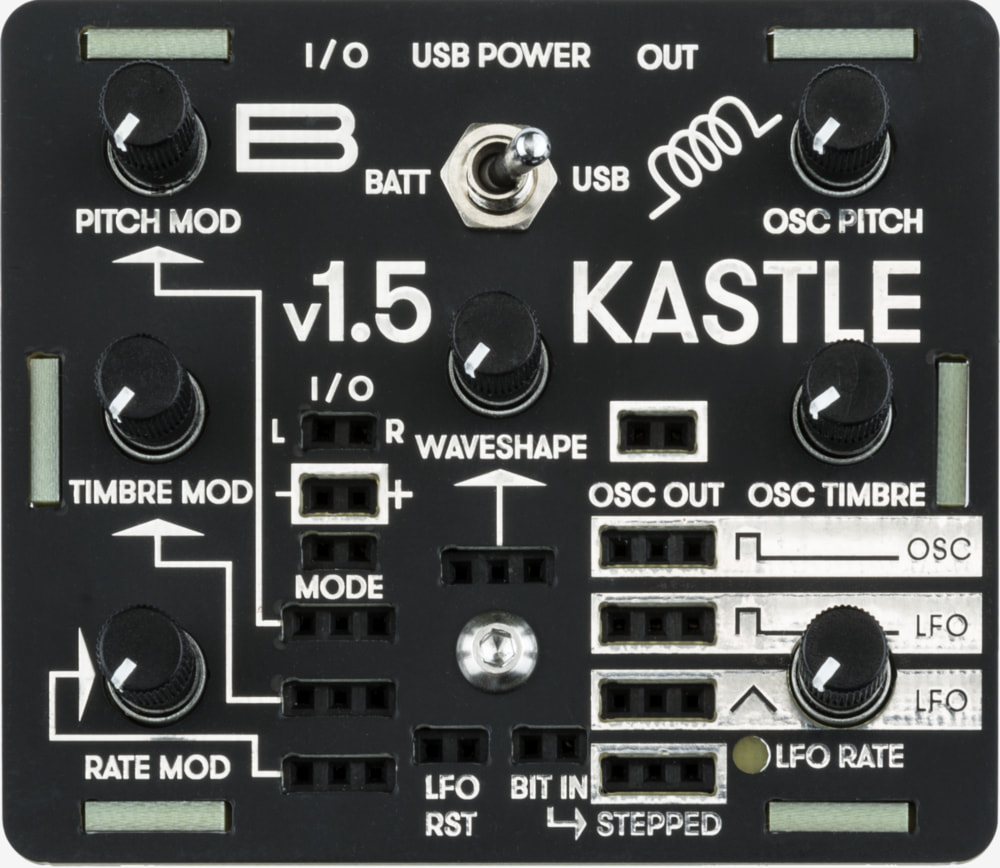
\includegraphics[width=0.75\linewidth,height=0.25\textheight,keepaspectratio]{images/bastl-kastle-v15.jpg}
  \caption{Bastl Instruments Kastle v1.5}
  \caption*{Retrieved from \cite{website-bastl-instruments-current}}
  \label{fig:bastl-kastle-v15}
\end{figure}

As of writing, 2 different units are in production, both retailing for ~100.00 USD, the Kastle v1.5 melodic / drone synthesizer, and the Kastle Drum, for rhythm. The only difference between these synthesizers is the firmware and the labels on the faceplate. The community is encouraged to write new firmware to modify their behavior. 

\begin{figure}[ht]
  \centering
  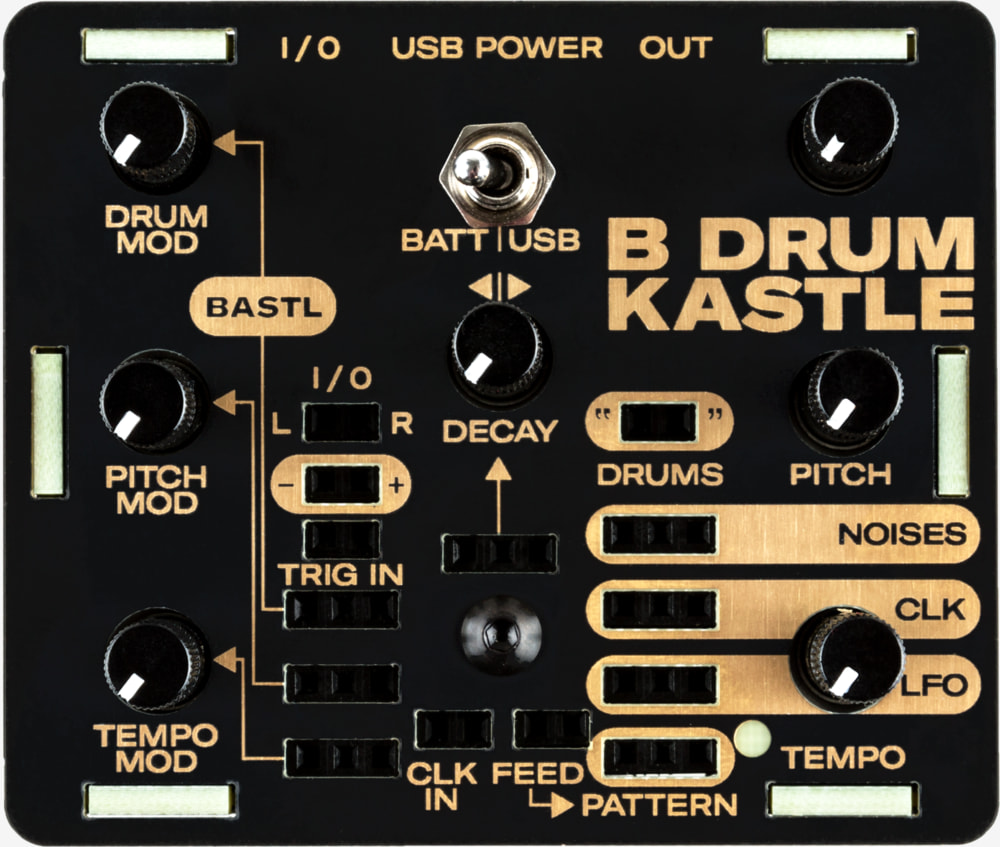
\includegraphics[width=0.75\linewidth,height=0.25\textheight,keepaspectratio]{images/bastl-kastle-drum.jpg}
  \caption{Bastl Instruments Kastle Drum}
  \caption*{Retrieved from \cite{website-bastl-instruments-current}}
  \label{fig:bastl-kastle-drum}
\end{figure}

Another instrument I want to highlight is the Illuminati, currently discontinued, a device that uses different inputs (audio, control voltage, \acrshort{MIDI} messages), to control the light intensity of connected USB lamps, which influenced the conception of Tiny trainable instruments as multimedia arts instruments, not only focusing on audio and music, but also printed text, light, and screen output.

\begin{figure}[ht]
  \centering
  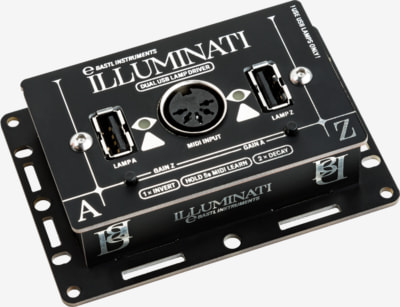
\includegraphics[width=0.75\linewidth,height=0.25\textheight,keepaspectratio]{images/bastl-illuminati.jpg}
  \caption{Bastl Instruments Illuminati}
  \caption*{Retrieved from \cite{website-bastl-instruments-current}}
  \label{fig:bastl-illuminati}
\end{figure}

The final instrument from this company that I want to highlight is the OMSynth, one of many collaborations with Casper Electronics. This device is an educational and maker circuit development tool for creating synthesizers, it includes basic fundamental blocks, such as battery power, audio input and output, potentiometers for attenuating and boosting signals, and a suite of parts kits for building devices including sequencers, oscillators, and samplers, on the included breadboard. Its release as a kit was also a direct influence in the release of Tiny trainable instruments as a kit with instructions.

\begin{figure}[ht]
  \centering
  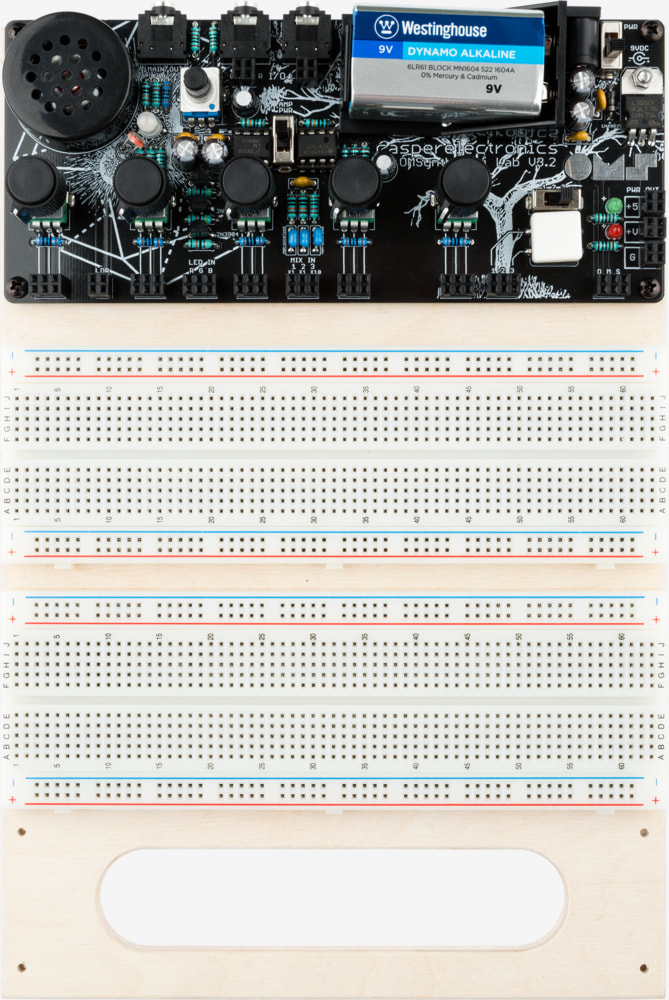
\includegraphics[width=0.75\linewidth,height=0.25\textheight,keepaspectratio]{images/bastl-omsynth.jpg}
  \caption{Bastl Instruments OMSynth}
  \caption*{Retrieved from \cite{website-bastl-instruments-current}}
  \label{fig:bastl-omsynth}
\end{figure}

Many BASTL standalone instruments are 200.00 USD or less, which is a huge contrast to the 1960s, when a Moog analog system II cost 6,200.00 USD, which was enough to buy a small house \cite{analog-days}. Also, many of their instruments are sold as kits for building and soldering them yourself, for the cheaper cost and the added educational aspect of having hands-on experience.

\subsection{Critter \& Guitari}

Critter \& Guitari is an American company based in Brooklyn NY, which have released in the past computational microcontroller-based audiovisual instruments, from which my favorite is the Kaleidoloop, currently discontinued. It is a sampler with an internal mic and speaker, that allows you to record audio and then control its output with 2 knobs for volume and playback rate. It is designed to be portable for doing field recordings, and it was an influence on the design of the Tiny trainable instruments library, which allows the construction of standalone instruments, that with a USB power bank or a battery, you can take for a walk or place anywhere you want.

\begin{figure}[ht]
  \centering
  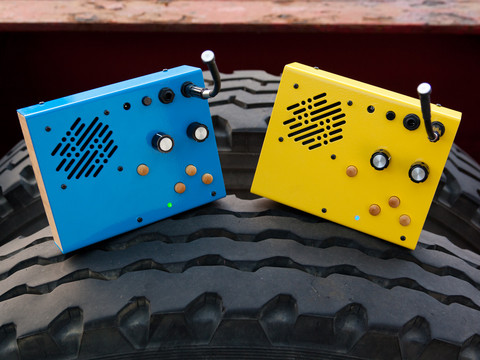
\includegraphics[width=0.75\linewidth,height=0.25\textheight,keepaspectratio]{images/critter-and-guitari-kaleidoloop.jpg}
  \caption{Critter \& Guitari Kaleidoloop}
  \caption*{Retrieved from \cite{website-critter-and-guitari-kaleidoloop}}
  \label{fig:critter-and-guitari-kaleidoloop}
\end{figure}

This company has released standalone scriptable computers for arts, which run Linux operating system + Pure Data software.

Organelle computer for sound, scriptable, Linux operating system + Pure Data software.

\begin{figure}[ht]
  \centering
  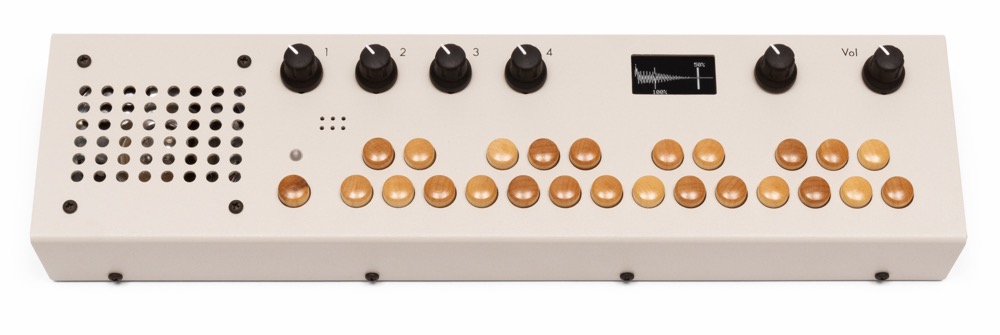
\includegraphics[width=0.75\linewidth,height=0.25\textheight,keepaspectratio]{images/critter-and-guitari-organelle-m.jpg}
  \caption{Critter \& Guitari Organelle M}
  \caption*{Retrieved from \cite{website-critter-and-guitari-current}}
  \label{fig:critter-and-guitari-organelle-m}
\end{figure}

ETC and EYESY computers for visuals, scriptable, Linux operating system + Python / pygame environment or openFrameworks.

\begin{figure}[ht]
  \centering
  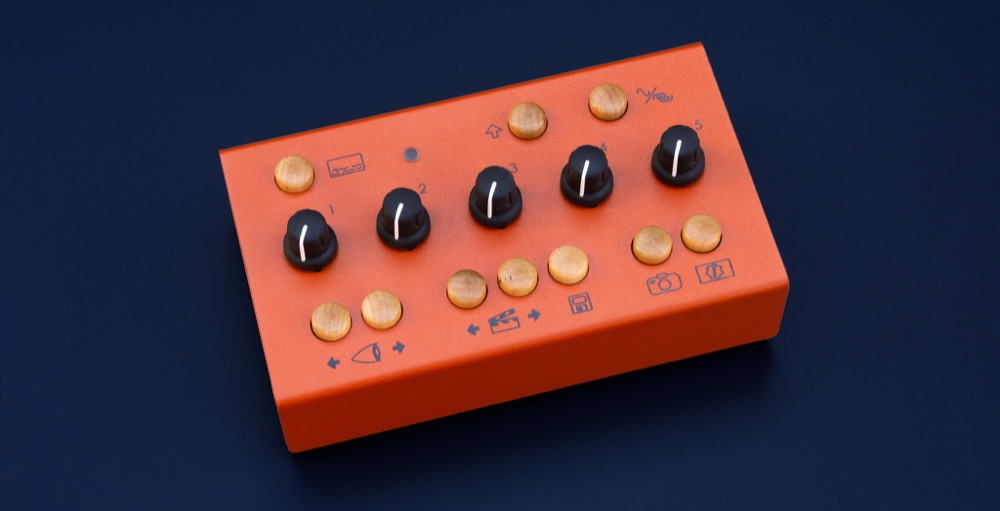
\includegraphics[width=0.75\linewidth,height=0.25\textheight,keepaspectratio]{images/critter-and-guitari-eyesy.jpg}
  \caption{Critter \& Guitari EYESY}
  \caption*{Retrieved from \cite{website-critter-and-guitari-current}}
  \label{fig:critter-and-guitari-eyesy}
\end{figure}

They can run on power supplies, and are also portable by the use of batteries.

\subsection{monome}

\begin{figure}[ht]
  \centering
  \includegraphics[width=0.75\linewidth,height=0.25\textheight,keepaspectratio]{images/monome-grid.jpg}
  \caption{monome grid}
  \caption*{Retrieved from \cite{website-monome-current}}
  \label{fig:monome-grid}
\end{figure}

Aleph: earlier sound computer.

Norns: sound computer, currently on its second iteration, with expanded hard drive. Also there is a \acrshort{DIY} version which is cheaper and runs on a Raspberry Pi.
Norns is a Linux machine, running SuperCollider for the sound engine, and Lua scripts. It has spawned a community that continually releases new scripts and software updates.

\begin{figure}[ht]
  \centering
  \includegraphics[width=0.75\linewidth,height=0.25\textheight,keepaspectratio]{images/monome-aleph.jpg}
  \caption{monome aleph}
  \caption*{Retrieved from \cite{website-monome-current}}
  \label{fig:monome-aleph}
\end{figure}

\begin{figure}[ht]
  \centering
  \includegraphics[width=0.75\linewidth,height=0.25\textheight,keepaspectratio]{images/monome-norns.jpg}
  \caption{monome norns}
  \caption*{Retrieved from \cite{website-monome-current}}
  \label{fig:monome-norns}
\end{figure}

\subsection{Shbobo}

In my first semester I was introduced by classmate Will Freudenheim to the Shbobo synthesizers by Peter Blasser. Peter Blasser has released several collections / companies of musical instruments, the most famous one being Ciat-Lonbarde.

\begin{figure}[ht]
  \centering
  \includegraphics[width=0.75\linewidth,height=0.25\textheight,keepaspectratio]{images/shbobo-shnth.jpg}
  \caption{Shbobo Shnth}
  \caption*{Retrieved from \cite{website-shbobo-current}}
  \label{fig:shbobo-shnth}
\end{figure}

\begin{figure}[ht]
  \centering
    \includegraphics[width=0.75\linewidth,height=0.25\textheight,keepaspectratio]{images/shbobo-shtar.jpg}
  \caption{Shbobo Shtar}
  \caption*{Retrieved from \cite{website-shbobo-current}}
  \label{fig:shbobo-shtar}
\end{figure}

Both run on microcontrollers, and they use a new proposed language called Shlisp, based on Lisp, and also they can be programmed using the Fish IDE.

As of 2021, their firmware and editor became open source, and it is available at \url{https://github.com/pblasser/shbobo}.

COMMENT ON OPEN SOURCE: something being open source doesn't necessarily mean it is accessible to a wider audience. Is one of the goals of your work to create instruments that are accessible to a wider audience?

They promote computer-centric approaches to making sound, such as the use of integers and metaphors of finite state machines, and also allow for different ways of playing and sensing, such as the use of antennas for detecting hand distance, a microphone for detecting speech and whistling, and wooden bars with piezos for detecting pressure.

TODO: write how this inspired the new interactions i am inventing or appropriating for Tiny trainable instruments, such as a drum machine you can talk to, Alexa spinoff.

\section{Education}

This thesis is inspired by the work of the research group Lifelong Kindergarten at MIT Media Lab, led by professor Mitchel Resnick. In the book with the same title, he builds on Seymour Papert’s work, and proposes that educational projects should have “Low floor, wide walls, high ceilings”, and that learners thrive when they engage in the 4 Ps: “Peers, projects, passion, play”.

In terms of peers, I have been lucky to have been supported by the MIT UROP office and MIT Media Lab, and had the opportunity to work with MIT undergrad researchers Peter Tone and Maxwell Wang. Also, this project was taught in collaborative workshops where people could discuss their ideas with their peers.

In terms of projects, this thesis includes the release of a software library, so that people can make the software their own, and spin-off their own projects. It is also open source so that people can learn from my mistakes and also fork to adapt to their needs.

In terms of passion, this thesis is 

In terms of play, this thesis project is not about correct answers, or even excellent classification with \acrshort{ML}, it's all about finding innovative ways to interact with multimedia material, celebrate the small victories and the big glitches, and iterate over and over again.

\section{Creative ML}

COMMENT: what is the main argument of the whole piece and how does each independent part connect to that? you should start with a story from previous experiences that is particularly relevant as to why you were inspired to do this work. think "papert and the gears"

While being a graduate student and research resident at \acrshort{NYU} \acrshort{ITP} I saw how quick things changed in terms of \acrshort{ML}. I saw how the project deeplearn.js allowed for people to train and deploy \acrshort{ML} on their browsers, and how this library was acquired by Google and repurposed as TensorFlow.js, a JavaScript version of their \acrshort{ML} framework TensorFlow.

In turn, at \acrshort{NYU} \acrshort{ITP} a team of artists and programmers built the library and community of ml5.js, with the 5 being an homage to p5.js. Technically, ml5.js is a wrapper for TensorFlow.js, in the same spirit that p5.js is a wrapper for HTML5 elements such as the canvas.

\begin{figure}[ht]
  \centering
    \includegraphics[width=0.75\linewidth,height=0.25\textheight,keepaspectratio]{images/sam-lavigne-training-poses.jpg}
  \caption{Sam Lavigne, Training Poses, 2018}
  \caption*{Retrieved from \cite{website-sam-lavigne-training-poses}}
  \label{fig:sam-lavigne-training-poses}
\end{figure}

The last spark that led me to this thesis was the release of 2 libraries for \acrshort{ML} on the Arduino platform: The currently beta version Arduino KNN, which allows for on-device training and resembles my earlier studies with Wekinator, in a more portable and private way, no data leaves the microcontroller, and the whole neural network can be wiped with one click of a button.

At a more complex level, I am also working with the TensorFlow Lite Micro, which I learned from Arduino blogs, and which currently is supported by the hardware Arduino Nano 33 \acrshort{BLE} Sense.

COMMENT TO THE ABOVE PARAGRAPH: you may not even need to include the specific details here, but just highlight in larger overviews the types of projects you've worked on or the educational fields that influence your work

In late 2020 and early 2021 I completed the just released series of 3 courses of the TinyML Professional Certificate by Harvard at the online platform edx.org

Newer books and references that this thesis was inspired by include the books “You Look Like a Thing and I Love You: How Artificial Intelligence Works and Why It's Making the World a Weirder Place” by Janelle Shane (2019), and the book “Making Pictures with Generative Adversarial Networks” by Casey Reas (2019).

Also Yining Shi created a new class at \acrshort{NYU} \acrshort{ITP} in 2020, at the intersection of \acrshort{ML} and physical computing.

\section{Digital rights}

\acrshort{ML} algorithms need data to be trained on. I think it’s a human right to not be surveilled, and I hope my thesis can put a positive spin on the gathering of data, by letting users perform auto surveillance, like the Ai Weiwei piece WeiweiCam, a 2021 project where the artist installed cameras for self surveillance as a protest against the Chinese government.

A huge inspiration for my thesis has been the Guardian Project by the Electronic Frontier Foundation, and the research and activism work by Sasha Sasha Costanza-Chock.

\section{Digital rights}

Electronic Frontier Foundation

Edward Snowden

Design Justice Network

\section{Opera of the Future projects}

During the development of this thesis, I have been fortunate to collaborate on different capacities with other thesis projects by classmates at Opera of the Future, which has directly inspired my work.

\subsection{Squishies, by Hannah Lienhard}

Squishies is Hannah Lienhard's master's thesis, and consists of novel squishable interfaces for musical expression. We shared discussions about low-level sound design, code reusability, sound art education, and digital instruments. We were part of a master's thesis working group, facilitated by Roya Moussapour with two other Media Lab classmates, where we workshopped drafts of our thesis. This practice and feedback has been critical in shaping the language and discourse of this thesis document.

\subsection{Fluid Music, by Charles Holbrow}

Fluid Music is Charles Holbrow's PhD thesis. It is a library for library design, documentation for contributors. The design of the interface, documentation, and scope of the thesis were a direct influence on the documentation and API coding style of this project.

Overall thoughts: I think it would be great if your Chapter 3 clearly led you to the design principles you lay out in Chapter 4. So, why is “open” important -> because of the collaborations or arduino libraries you used. Why is “cheap”/”privacy” -> coded bias and ability to tinker, etc.


TODO: mention the impact of the documentary Coded Bias, and how these researchers impacted my desire to make my thesis. Also mention how right before pandemic I had started a pottery class, with the intention of making clay-based instruments for thesis, as a metaphor of making code and hardware and software feel fluid and not static, I want to empower people to program, in particular \acrshort{ML} because of its dangerous implementations by oppressive governments and corporations, and in particular for arts, for making artists dream come true.

\chapter{Project evaluation}

\epigraph{Yeah you wanted a hit \\ but tell me \\ where's the point in it?}{You Wanted a Hit \\ LCD Soundsystem, 2010}

\section{Digital release}

This thesis project lives on 2 different repositories, hosted on GitHub, to foster collaboration via issues and pull requests, and also with frequent updates, to show people the whole process behind this thesis project.

The main repository contains this thesis document, Jupyter notebooks for machine learning, documentation for beginners and educators, and auxiliary shell scripts. It is hosted at \url{https://github.com/montoyamoraga/tiny-trainable-instruments}.

The auxiliary repository contains the Arduino library, including its source code and examples. It is hosted at \url{https://github.com/montoyamoraga/TinyTrainable}.

\section{Workshop}

\begin{figure}[ht]
  \centering
  \includegraphics[width=0.75\linewidth,height=0.25\textheight,keepaspectratio]{images/workshop-packages.jpg}
  \caption{Workshop packages}
  \caption*{Picture by myself}
  \label{fig:workshop-packages}
\end{figure}

For user testing and sharing this thesis, some workshops were conducted during TODO, with support from a grant at CAMIT for teaching the workshops in English in USA, and in Chile in Spanish, remotely over teleconferencing software and after being approved by the MIT COUHES TODO explain.

The workshop instructions are documented on the docs/ folder of the repository available at \url{https://github.com/montoyamoraga/tiny-trainable-instruments}

Each workshop consists of 2 sessions of 2 hours each, spread over 2 consecutive days.

In the first session we will first help people with installation of the software, and then move on to start wiring the materials on the electronic breadboard material. We will concentrate on the simpler examples with color input. We will also collect data of gesture and speech to create custom databases and use them to train other slow machine learning models that will keep on running on the student's workshops after the workshop is over.

In the second session we will use the result of the trained models to create more advanced instruments that react to gesture and speech. We will also show the participants the other 

I applied to and was awarded a grant by the Council for the arts at MIT (CAMIT), which consisted of 2,000.00 USD to buy materials to teach the Tiny Trainable Instruments workshop to 20 people, during June 2021.

I taught this workshop 3 times, 2 of them were in English for people based in the USA, and 1 time in Spanish for people based in Chile, with a total of 20 kits being delivered.

\begin{figure}[ht]
  \centering
  \includegraphics[width=0.75\linewidth,height=0.35\textheight,keepaspectratio]{images/workshop-en-1.jpg}
  \caption{Workshop flyer cover in English}
  \caption*{Graphics by Renata Gaui}
  \label{fig:workshop-english-flyer-page-1}
\end{figure}

\begin{figure}[ht]
  \centering
  \includegraphics[width=0.75\linewidth,height=0.35\textheight,keepaspectratio]{images/workshop-es-1.jpg}
  \caption{Workshop flyer cover in Spanish}
  \caption*{Graphics by Renata Gaui}
  \label{fig:workshop-spanish-flyer-page-1}
\end{figure}

The multimedia aspect of this project was featured, in particular the ability to use different inputs, including color, gesture and speech, to control different outputs, including serial messages, sound, and motor movement.

\begin{figure}[ht]
  \centering
  \includegraphics[width=0.75\linewidth,height=0.35\textheight,keepaspectratio]{images/workshop-en-2.jpg}
  \caption{Workshop multimedia output in English}
  \caption*{By Renata Gaui}
  \label{fig:workshop-english-flyer-page-2}
\end{figure}

\begin{figure}[ht]
  \centering
  \includegraphics[width=0.75\linewidth,height=0.35\textheight,keepaspectratio]{images/workshop-es-2.jpg}
  \caption{Workshop multimedia output in Spanish}
  \caption*{By Renata Gaui}
  \label{fig:workshop-spanish-flyer-page-2}
\end{figure}

\section{Multimedia documentation}

TODO: upload a collection of examples made by people who came to the workshops, featuring the software library and what they learned.

\chapter{Conclusions and future work}

\epigraph{Don't get any big ideas \\ they're not gonna happen}{Nude \\ Radiohead, 2007}

In this thesis I have presented all the stages of the design and development of a software library for creating new standalone multimedia instruments using machine learning and microcontrollers, with a strong focus on AI ethics. The project includes software examples, hardware suggestions, educational material, and strategies for ethical off-cloud machine learning and creation of custom artisanal databases.

This thesis is also the basis for further research, including the creation of subsequent multimedia instruments and software libraries, the writing of new courses and educational units at the intersection of arts, physical computing, interaction design, and computational ethics.

\section{Contributions}

Concrete contributions:

\begin{enumerate}
  \item Publishing TinyTrainable, a software library for machine learning with microcontrollers for multimedia art.
  \item Design, writing, and teaching a 4 hour workshop for beginners, enthusiasts, and artists to teach with the software library.
  \item Publishing code and tutorials for creating custom databases for gesture and speech.
  \item Publishing custom trained machine learnign models for gesture and speech recognition.
  \item Publishing code and tutorials for training machine learning algorithms on the cloud and on personal computers for privacy and agency.
  \item Publishing other related software libraries, such as MaquinitasParams for communication with other instruments, and MaquinitasRitmos for rhythmic data.
\end{enumerate}

Abstract contributions:

\begin{enumerate}
 \item Demonstrating how a broader range of people can use machine learning to support their creative expression." Or do think it's better to focus on more "concrete" descriptions of contributions?
\end{enumerate}

\section{Lessons learned}

\begin{enumerate}
  \item Writing software for artists is hard, publishing as a library for other artists is even harder.
  \item Collaboration with other people is essential to write usable code and educational material.
  \item Document all design decisions to explain why and how everything works.
\end{enumerate}

\section{Future work}

\subsection{Hardware for new instruments}

This thesis relies on an Arduino microcontroller because of their open source nature, commercial availability, software and community support, and detailed documentation.

In particular I picked the Arduino Nano 33 BLE Sense, because of 2 main reasons at the time this project started in late 2020: it is the only Arduino supported by TensorFlow Lite for microcontrollers and featured in the HarvardX certificate on Tiny Machine Learning, and also because of its convenience of having embedded sensors, which makes it simpler and cheaper to acquire data for live interaction and for building custom databases, eliminating barriers to instruments makers and prototypers.

Microcontrollers come and go, most probably this board will be discontinued, but the strategies and software can be forked and adapted to other microcontrollers and software architectures. I am particularly looking forward to adapt this thesis project to other open source microcontrollers, including other Arduino boards, PJRC Teensy and Adafruit Circuit Playground, which would enable the adoption of other software stacks, such as Python instead of C++, and also to other communities building multimedia instruments and experiences.

In terms of the outputs of the Tiny trainable instruments, I focused on creating many parallel multimedia approaches, including making sounds with piezo buzzers and MIDI, manipulating light with LEDs, creating movement and rhythm with servo motors, and printing text with thermal printers and screens. This is to appeal to a larger audience of artists and learners, interested in different mediums, and I hope this thesis project inspires more complex artworks and interactive experiences that this library currently allows, and that people can contribute back to the library to share these new capabilities with everyone.

The Tiny trainable instruments are built with prototyping electronic breadboards, to make explicit their open-endedness, and to promote experimentation and lower barriers. A further iteration of this project would include the creation of custom printed circuit boards with fixed wiring, and also enclosures and packaging.

\subsection{Software for new instruments}

This thesis has been published as an open source software library for Arduino. It promotes modularity and adaptability, where a Tiny Trainable Instrument can be any combination of the multiple inputs and outputs.

The file structure of the source code and the software dependencies of this library was also built with flexibility in mind, to encourage the remix and adaptation of this library to further projects.

A challenging aspect of this project is the breadth of the disciplines combined, and its novel application of machine learning in microcontrollers. As discussed in previous chapters, there is a trend and new wave of builders and makers creating standalone multimedia instruments, based on open operating systems like Linux, and/or different microcontrollers. 

Despite the existence of artists and makers building standalone computational instruments, these skills are still hard to acquire. Additionally, the principles of this project, including being as cheap as possible, and as open as possible, are designed to encourage experimentation and hacking, but also can pose additional challenges. I hope this project encourages people to learn how to make instruments, and also engages in discourse about the creation of new curricula for the next generation of instrument makers and artists.

Another challenging aspect of writing software for multimedia instruments is its licensing, both choosing a license and also respecting and understanding the license of other code and resources we are using. The dependencies of this software are mostly other libraries by Arduino, Google, Adafruit, and with different licenses including public domain, MIT, and Apache. I hope this document helps to navigate these legal complexities and that this project helps artists and enthusiasts to navigate this landscape and overcome these barriers.

\subsection{Educational impact}

This project was built to inspire and celebrate a new generation of coursework, workshops, books, in the disciplines of ethical machine learning and microcontroller-based instruments.

I hope that this thesis project is adopted by educators, to introduce students to machine learning, physical computing, media arts, and ethics.

Many sections of this project could be adapted to further existing curricula for music, rhythm, ethics, computer science, and to create a new wave of instrument makers and media artists.

I hope to see new classes taught in high school, universities, and cultural centers, at the intersection of multimedia art, physical computing, and ethical machine learning.

\appendix
\chapter{Context}

\epigraph{You might have to think  of \\ how you got started \\ sitting in your little room}{Little Room \\ The White Stripes, 2001}

Since joining MIT in summer 2019 I didn't leave the USA, and it's the longest stretch I have had of not visiting my home country Chile. This thesis in particular was written between November 2020 and August 2021, mostly in Boston MA USA, while on a F-1 visa.

\section{Language}

My native language is Spanish, and this thesis was written in English, using the metric system, and the Gregorian year-month-day format.

I tried to avoid violent language, including some widespread conventions on computer science which I hope become obsolete, such as executing a file, instead of running a file.

\section{Software}

This thesis document was written using LaTeX and the Microsoft Visual Studio Code editor, and then exported to the PDF format.

The TinyTrainable library was written in C++, and packaged as an Arduino library, relying on open source library dependencies by Adafruit, Arduino, and Google.

The auxiliary code is a mix of Python scripts, Jupyter Python notebooks, and shell scripts.

The documentation was written using Markdown.

The workshops were taught using the videoconferencing software Zoom, and organized via Google Forms.

\section{Hardware}

This project was written on a 2017 Macbook Air 13-inch, running the macOS 10.15.7 Catalina operating system.

The software library and the software examples were written to be deployed on the Arduino Nano 33\acrshort{BLE}Sense microcontroller.

\section{Collaborators}

Priscilla Capistrano is the senior administrative assistant at the Opera of the Future research group and made sure that everything worked.

Peter Tone is a MIT undergraduate student, who was a researcher, designer, programmer, and tester of the TinyTrainable Arduino library, as part of the MIT UROP program.

Maxwell Wang is a MIT undergraduate student who was a documentation writer, and hardware and software tester, as part of the MIT UROP program.

Roy Macdonald solved my most difficult programming questions, and helped to implement the solutions.

The Council for the Arts at MIT provided the generous funding of the workshop materials.

Renata Gaui designed and created the flyers for the workshops.

Bernardita Moraga packaged and distributed the materials for the workshop in Chile.

\newpage

\chapter{Scripts}

\epigraph{By pressing down a special key \\ it plays a little melody}{Pocket calculator \\ Kraftwerk, 1981}

During the writing of this thesis I developed scripts, which are included in this repository on the folder scripts.

I abstracted them to make them useful for other people and published them with a MIT License at https://github.com/montoyamoraga/scripts.

Since they are useful scripts and they are commented, I include them here.

\section{Formatting code with clang-format}

clang-format is a command line tool for formatting code. This script was written to auto format the code from the Arduino/C++ library TinyTrainable.

\lstinputlisting[language=bash]{../scripts/clang-format.sh}

\section{Converting formats with ffmpeg}

ffmpeg is a command line tool for converting audiovisual files between formats. This script was written to convert audio files from .mp3 to .ogg format for training a database for speech recognition.

\lstinputlisting[language=bash]{../scripts/ffmpeg-convert.sh}

\section{Deleting metadata with exiftool}

exiftool is a command line tool for reading and writing metadata from files. This script was written to delete metadata from images, like GPS coordinates added by modern smartphones, only keeping the actual image.

\lstinputlisting[language=bash]{../scripts/exiftool-delete-metadata.sh}

\section{Converting formats with pandoc}

pandoc is a command line tool for converting between formats. This script was written to convert from .tex files to .docx files, so that each chapter of this thesis document could be uploaded to Google Docs for feedback from the committee.

\lstinputlisting[language=bash]{../scripts/pandoc-convert.sh}

\chapter{Documentation}

% \epigraph{By pressing down a special key \\ it plays a little melody}{Pocket calculator \\ Kraftwerk, 1981}

For this thesis I wrote the following documentation, included at the docs/ folder of the repository, and also included here.

\includepdf[pages=-,pagecommand={}]{./../docs/en/0-bill-of-materials.pdf}

\includepdf[pages=-,pagecommand={}]{./../docs/en/1-installation.pdf}

\includepdf[pages=-,pagecommand={}]{./../docs/en/2-wiring.pdf}

\chapter{Open source contributions}

During this thesis I contributed the following \glspl{pull-request} to open source projects that are either direct dependencies or inspirations.

\begin{table}[ht]
    \centering
    \begin{tabular}{ | l | l | l |}
        \hline
        Author & Repository & Contribution \\
        \hline
        Adafruit & \cite[Adafruit{\_}SSD1306]{repository-adafruit-adafruit_ssd1306} & \cite[Format binary numbers]{pull-request-adafruit-adafruit_ssd1306} \\
        \hline
        tinyMLx & \cite[TinyMLx Arduino Library]{repository-tinymlx-arduino-library} & \cite[Update architecture name]{pull-request-tinymlx-arduino-library} \\
        \hline
        Yining Shi & \cite[ML for Physical Computing]{repository-yining1023-machine-learning-for-physical-computing} & \cite[Fixed some typos]{pull-request-yining1023-machine-learning-for-physical-computing} \\
        \hline
    \end{tabular}
    \caption{Pull requests to open source projects}
    \label{table:open-source-pull-requests}
\end{table}{}

For more information and thoughts about the communities and practice of developing and maintaining open source software for artists, I recommend reading the \acrfull{OSSTA} report, available online at \cite{website-repository-ossta-report}, by Lauren Lee McCarthy, Thomas Hughes, and Golan Levin.

\chapter{Rules of thumb}

\epigraph{Wishes on a wheel \\ How it's supposed to feel}{Wishes \\ Beach House, 2012}

During this thesis I have tried to follow these rules of thumb:

\begin{itemize}
  \item Openly share small steps
  \item Learn by failing often
  \item Contribute back
  \item Use tools you like
  \item Cite other people
  \item Sleep as much as possible
\end{itemize}

%% This defines the bibliography file (main.bib) and the bibliography style.
%% If you want to create a bibliography file by hand, change the contents of
%% this file to a `thebibliography' environment.  For more information 
%% see section 4.3 of the LaTeX manual.
\begin{singlespace}
% \printbibliography
\bibliography{main}
% \bibliographystyle{plain}
\bibliographystyle{unsrt}
\end{singlespace}

\end{document}
